
\documentclass[sigconf]{acmart}

%%%
%%% \BibTeX command to typeset BibTeX logo in the docs
%%\AtBeginDocument{%
%% \providecommand\BibTeX{{%
%% \normalfont B\kern-0.5em{\scshape i\kern-0.25em b}\kern-0.8em\TeX}}}



\copyrightyear{2019}
\acmYear{2019}
\setcopyright{acmlicensed}
\acmConference[ICPP '19]{ICPP 2019: 48th International Conference on Parallel Processing}{August 05--08, 2019}{Kyoto, Japan}
%%\acmBooktitle{Woodstock '18: ACM Symposium on Neural Gaze Detection, June 03--05, 2018, Woodstock, NY}
%%\acmPrice{15.00}
%%\acmDOI{10.1145/1122445.1122456}
%%\acmISBN{978-1-4503-9999-9/18/06}

\usepackage{graphicx} 

\usepackage[utf8]{inputenc}
%%\usepackage{amsmath}
%%\usepackage{amsthm}
\usepackage{amssymb}
\usepackage{threeparttable}
\usepackage{graphicx}
\usepackage{color}
\usepackage{paralist}
\usepackage{framed}
\usepackage{caption}
%%\usepackage{subcaption}
\captionsetup{compatibility=false}
\usepackage{todonotes}
\usepackage{subfig}
\usepackage{multirow}
\usepackage{dblfloatfix}

\usepackage[shortlabels]{enumitem}



\usepackage{algorithmic}
\usepackage[ruled,vlined]{algorithm2e}
%%\usepackage[cmex10,fleqn]{amsmath}
\usepackage{amsfonts}

%%to comment all todos
%%\renewcommand{\todo}{}


\SetKw{continue}{continue}

\usepackage{tikz}
\usetikzlibrary{fit,calc,positioning,decorations.pathreplacing,matrix}


\definecolor{pdfurlcolor}{rgb}{0,0,0.6}
\definecolor{pdfcitecolor}{rgb}{0,0.6,0}
\definecolor{pdflinkcolor}{rgb}{0.6,0,0}
\usepackage{epsfig,color}
%\usepackage[colorlinks=true,citecolor=pdfcitecolor,urlcolor=pdfurlcolor,linkcolor=pdflinkcolor,pdfborder={0 0 0}]{hyperref}


%%\newcommand{\scomm}{\ensuremath{{\cal S}_{\text{COMM}}}}
%%\newcommand{\scomp}{\ensuremath{{\cal S}_{\text{COMP}}}}


\newcommand{\scomm}{\ensuremath{{S}_{\text{COMM}}}}
\newcommand{\scomp}{\ensuremath{{S}_{\text{COMP}}}}
\newcommand{\threepart}{\textsc{3Par}\xspace}

% Command for figures

\tikzset{xtick/.style={inner xsep=0pt, inner ysep=3pt, minimum
		size=0pt, draw, label=below:#1},%
	comm/.style args={#1start#2length#3color#4}{rounded corners=1mm, draw, inner
		sep=0pt, fill=#4, label=center:#1, fit={(#2,0.75)
			(#2+#3,1.5)}},%
	comp/.style args={#1start#2length#3color#4}{rounded corners=1mm, draw, inner
		sep=0pt, fill=#4, label=center:#1, fit={(#2,0)
			(#2+#3,0.75)}},%
}

\newcommand{\schedule}[3]{
	\draw[->] (-0.2, 0) -- (#1, 0) node[below] {$t$};
	\draw (0, 0) -- (0, 1.5);
	\node at (-0.8, 0.75)[rotate=90] {#2};
	\draw[dashed,gray] (0, 0.75) -- (#1, 0.75);
	\foreach \t in {0,#3} {
		\node[xtick=\t] at (\t, 0){};
	}
}
\newcommand{\task}[6][0]{
	\node[comm=#2 start #3 length #4 color #6]{};
	\node[comp=#2 start #3+#4+#1 length #5 color #6]{}; 
}



%%\newtheorem{theorem}{Theorem}
%%\newtheorem{corollary}{Corollary}[theorem]
%\newtheorem{lemma}[theorem]{Lemma}

%%\pagenumbering{gobble}

\begin{document}
	
	\title{Performance Models for Data Transfers: A Case Study with Molecular Chemistry Kernels}
	
	\author{Suraj Kumar}
	\affiliation{%
		\institution{Pacific Northwest National Laboratory}
		\city{Richland, Washington, USA}}
	\email{suraj.kumar@pnnl.gov}
	
	
	
	\author{Lionel Eyraud-Dubois}
	\affiliation{\institution{Inria Bordeaux -- Sud-Ouest}\institution{Université de Bordeaux, France}}
	\email{lionel.eyraud-dubois@inria.fr}
	
	\author{Sriram Krishnamoorthy}
	\affiliation{
		\institution{Pacific Northwest National Laboratory}
		\city{Richland, Washington, USA}}
	\email{sriram@pnnl.gov}
	
	\renewcommand{\shortauthors}{Kumar and Eyraud-Dubois, et al.}
	
	
	%
	% The abstract is a short summary of the work to be presented in the article.
	\begin{abstract}
		%%		\todo[inline]{Initial submission deadline: April 15}
		With increasing complexity of hardwares, systems with different memory nodes are ubiquitous in High Performance Computing (HPC). It is paramount to develop strategies to overlap the data transfers between memory nodes with computations in order to exploit the full potential of these systems. In this paper, we consider the problem of deciding the order of data transfers between two memory nodes for a set of independent tasks with the objective to minimize the makespan. We prove that with limited memory capacity, obtaining the optimal order of data transfers is a NP-complete problem. We propose several heuristics for this problem and provide details about their favorable situations. We present an analysis of our heuristics on traces, obtained by running 2 molecular chemistry kernels, namely, Hartree–Fock (HF) and Coupled Cluster Single Double (CCSD) on 10 nodes of an HPC system. Our results show that some of our heuristics achieve significant overlap for moderate memory capacities and are very close to the lower bound of makespan.
	\end{abstract}
	
	%%\begin{CCSXML}
	%%	<ccs2012>
	%%	<concept>
	%%	<concept_id>10010520.10010553.10010562</concept_id>
	%%	<concept_desc>Computer systems organization~Embedded systems</concept_desc>
	%%	<concept_significance>500</concept_significance>
	%%	</concept>
	%%	<concept>
	%%	<concept_id>10010520.10010575.10010755</concept_id>
	%%	<concept_desc>Computer systems organization~Redundancy</concept_desc>
	%%	<concept_significance>300</concept_significance>
	%%	</concept>
	%%	<concept>
	%%	<concept_id>10010520.10010553.10010554</concept_id>
	%%	<concept_desc>Computer systems organization~Robotics</concept_desc>
	%%	<concept_significance>100</concept_significance>
	%%	</concept>
	%%	<concept>
	%%	<concept_id>10003033.10003083.10003095</concept_id>
	%%	<concept_desc>Networks~Network reliability</concept_desc>
	%%	<concept_significance>100</concept_significance>
	%%	</concept>
	%%	</ccs2012>
	%%\end{CCSXML}
	\ccsdesc[100]{Computer systems organization~ High Performance Computing }
	\ccsdesc[100]{Computing Methodologies~Modeling and Simulation}
	\ccsdesc[100]{General ~ Performance}
	
	
	\keywords{Communication Scheduling, Memory Nodes, Runtime Systems, Communication-Computation Overlap, Molecular Chemistry}
	
	\maketitle
	
	\section{Introduction}
	\label{sec:intro}
	
	With the advent of multicore, and the use of accelerators, it is notoriously cumbersome to exploit the full capability of a machine. Indeed, there are several challenges that come into picture. First, every architecture provides its own efficacy and interface. Therefore, a steep learning curve is required for programmers to take good utilization of all resources. Second, scheduling is a well known NP-Complete optimization problem, and hybrid and distributed resources make this problem harder (we refer ~\cite{webpagescheduling} for a survey on the complexity of scheduling problems and ~\cite{bleuse2015scheduling} for a recent survey in the case of hybrid nodes). Third, due to shared buses and parallel resources, it is challenging to obtain a precise model based on prediction of computation and communication times. Fourth, the number of architectures has increased drastically in recent years, therefore it is almost impossible to develop hand tuned optimized code for all these architectures. All these observations led to the development of different task based runtime systems. Among several runtimes, we may cite QUARK~\cite{YarKhan:2011:Quark:Manual} and PaRSEC~\cite{parsec} from from ICL, Univ. of Tennessee Knoxville (USA), StarPU~\cite{starpu} form Inria Bordeaux (France), Legion~\cite{legion12} from Stanford Univ. (USA), StarSs~\cite{ompss} from Barcelona Supercomputing Center (Spain), KAAPI~\cite{kaapi} from Inria Grenoble (France). All these runtime systems allow programmers to express their algorithms at the abstract level in the form of direct acyclic graphs (DAG), where vertices represent computations and edges represent dependencies among them. Sometimes some static information is also provided along with the DAG, such as distance to exit (last) node as a priority or affinity of computation towards resources. The runtime is then responsible for managing scheduling of computations and communications, data transfers among different memories, computation-communication overlap, and load balance.
	
	
	%%	Historically there is a great focus on the design of parallel algorithms and to minimize the complexity of the computations. Also In the last decade, there is a drastic improvement in the hardware to provide perminent rate of computation, but little improvement has been achieved for the rate of data movement. With extreme scale computing, supercomputers face bottlenecks due to ever growing need of data. Therefore focus of HPC community is now changing towards avoiding, hiding and minimizing communications. (Kyelick work and http://science.energy.gov/~/media/ascr/ ascac/pdf/meetings/20140210/Top10reportFEB14.pdf )
	
	
	In the last few decades, we have witnessed a drastic improvement in the hardware to provide higher rate of computation, but comparatively smaller improvement has been achieved for the rate of data movement. With extreme scale computing, supercomputers face bottlenecks due to the need of large amount of data~\cite{ascaccommitteereport2014,yelick2016}. Therefore, the HPC community is now focusing on avoiding, hiding and minimizing communication costs.
	
	
	Certain applications such as dense linear algebra kernels have regular structure. Therefore, it is possible to associate priorities to computations, based on the task graph structure, and to use them at runtime to make the execution efficient. In irregular applications, programmers do not know the precise structure of the task graphs in advance: tasks are added recursively based on certain sentinel constraints. For such applications, the runtime system sees a set of independent tasks and schedules them on different processing units. It is extremely important for runtimes to decide the order of data transfers for these scheduled computations so as to maximize the overlap between computations and communications. This is the main topic of this paper. We prove that the order of communications on two memory nodes with the objective of minimizing the makespan is a NP-Complete problem if the memory of the target node is limited. Our proof is inspired from work by~\cite{Papadimitriou:1980:FSL:322203.322213}, which applies a similar technique for 2-machine flowshop problem with bounded capacity. The main difference between both approaches is that they consider all tasks have the same occupation on the second machine and the memory occupation starts when the processing finishes on the first machine. On the contrary, our approach is designed for tasks appearing in scientific workloads whose memory requirements are highly irregular and we consider that memory is acquired before starting the data transfer on the communication resource. We propose different runtime strategies in order to maximize the overlap of computations and communications. We evaluate our strategies on the context of a cluster of homogeneous nodes. However, our approach is generic and easily adaptable to any system which operates on different memory spaces. Here are the important contributions of this paper:
	
	
	\renewcommand{\labelitemi}{$\bullet$}
	\begin{itemize}
		\item NP-Completeness proof for the general data-transfer problem 
		\item Proposed different scheduling strategies with the objective to minimize the makespan
		%%		\item An optimal strategy and its proof, when there is not any memory capacity constraint on the target machine
		\item Linear programming formulation of the problem
		\item Numerous experiments to assess the effectiveness of our strategies on molecular chemistry kernels 
	\end{itemize}
	
	The outline of the paper is the following. Section~\ref{sec:relatedWork} describes past work on the computations with limited memory and similar problems in the literature. In section~\ref{sec:theoreticalProof}, we present an algorithm to obtain the order of data transfers when there is not any memory capacity restriction. Then, we also prove that in general data transfer problem is NP-complete. In Section~\ref{sec:heuristics}, we propose several heuristics and describe their favorable scenarios. We mainly consider three categories of heuristics: static heuristics, dynamic heuristics and static heuristics with dynamic corrections. Sections~\ref{sec:expSetting} describes our experimental setup and we evaluate our proposed strategies on two molecular chemistry kernels in Section~\ref{sec:expResults}. Our results show that static heuristics with dynamic corrections achieve good performance in most cases. We finally propose conclusions and perspectives in Section~\ref{sec:conclusion}.
	
	\section{Related Work}
	\label{sec:relatedWork}
	
	Historically there has been a great emphasis on the development of parallel algorithms and minimizing the complexity of computations. As the number of computation cores has increased drastically in recent years, supercomputers face bottleneck due to communication required by an application. Hence, in recent years the focus has changed towards developing communication avoiding algorithms, strategies to hiding communications and minimizing the data accessed by applications~\cite{yelick2016}. 
	
	
	The problem of scheduling tasks has been highly studied in the literature and many formulations are known to be NP-Complete~\cite{GareyJohnson}. Many static and dynamic strategies have been proposed and analyzed for scheduling tasks on heterogeneous resources~\cite{heft-Topcuoglu,hipc16multiresource,ipdps16starpu}. There is also a number of studies in the direction of task scheduling with the emphasis on improving locality and minimizing the communication cost~\cite{starpu,heft-Topcuoglu}. Stanisic et. al~\cite{luka-dmdar} proposed a heuristic to schedule tasks on a computational resource where most of its data is available. A similar approach has been adopted by Agullo et. al for the scheduling of sparse linear algebra kernels~\cite{agullo_fmm}. Predari et. al proposed heuristics to partition the task graph across a number of processors such that inter-processor communication can be minimized~\cite{predari:tel-01518956}.
	
	The problem considered in this paper also can be viewed as a flow shop problem: the communication link can be seen as a processing resource, and each task needs to first be handled by the communication link and then by the computational resource. Communication and computation times of a task can thus be considered as processing times on different machines. Johnson has provided scheduling strategies for 2 and 3-machine flow shop problems with infinite memory capacity~\cite{johnson}. 2-machine flow shop problem with finite buffer has been proven NP-Complete by Papadimitriou et. al~\cite{Papadimitriou:1980:FSL:322203.322213}, in which a constraint is imposed on the number of tasks that can await execution on the second machine.
	
	A number of other studies have focused on scheduling with limited memory and storage, starting with the work of register allocation for arithmetic expressions by Sethi and Ulman~\cite{Sethi:1970:GOC:321607.321620}. Sarkar et. al worked on the scheduling of graphs of smaller-grain tasks with limited memory, where each task requires homogeneous data size~\cite{vsarkar-pact}. The same work has been extended by Marchal et. al for task graphs where memory requirement of each task is highly irregular~\cite{loris-ipdps18}.
	
	
	%	\todo[inline]{theoretical/performance work on molecular chemistry kernels}
	
	%%	\section{Data Transfer Problem Formulation}
	\section{Problem Formulation}
	\label{sec:theoreticalProof}
	
	To exploit the full potential of a system it may be necessary to execute tasks on processing
	units where all of their data does not reside. A task may require all of its input data
	in local memory before starting the computation. There may be multiple tasks
	scheduled on a processing unit, which require to transfer data from the same
	memory node. Ordering data transfers for such tasks is very crucial for the
	communication-computation overlap, thus for the overall
	performance. In general, order of task execution with input
	and output data transfers can be  
	viewed as a 3-machine flowshop problem, where processing time on the first machine is 
	input data transfer time, processing time on the second machine is task computation time, 
	and processing time on the third machine is output data transfer time; and the objective is 
	to minimize the total makespan. This is a well known NP-complete problem~\cite{3machineFlowShopNPComplete}.
	
	
	In many cases, output data that needs to be retrieved after task execution is much smaller than the input data. It is often the case that future tasks running on the same memory node require output data of the past tasks. Therefore, most runtime systems transfer data to other memory nodes based on the demand -- not immediately after they were produced. It is also possible that all output data can be stored in a preallocated separate buffer on a memory node. Hence, we do not consider output data explicitly in our analysis and assume that output data is negligible or stored in a separate buffer for each task. Thus problem considered here is more similar to a 2-machine flowshop problem. We prove that ordering the execution of such tasks with finite memory capacity is a NP-complete problem: %%We also present an optimal algorithm to determine the order of execution of tasks when there is not any restriction on memory limit.
	
	%%	\todo[inline]{Find a citation saying 3-machine flowshop problem is NP-Complete.}
	%%%%	done:\todo[inline]{Rewrite both paragraphs together.}
	%%	In general, order of task execution with input and output data transfers can be 
	%%	viewed as 3-machine flowshop problem, where processing time on 1st machine is 
	%%	input data transfer time, processing time on 2nd machine is task execution time, 
	%%	processing time on 3rd machine is output data transfer time and the objective is 
	%%	to minimize the total makespan. This is a well known hard problem~\cite{NPComplete3Machine,johnson}. As stated earlier, we do not consider output data separately in our analysis and assume that output data is negligible or stored in a separate buffer. Hence, problem considered in this article is simpler than general 3-machine flowshop problem.
	
	\noindent\textbf{Problem $DT$} : A set of tasks $ST=\{T_1,
	\cdots, T_n\}$ is scheduled on a processing unit $P$ with
	memory unit $M$ of capacity $C$. Input data for tasks of $ST$
	reside on another memory unit $M'$. $COMM_i$ is the communication time to
	transfer input data from $M'$ to $M$ for task $i$ and $COMP_i$
	is the computation time of task $i$ on $P$. We assume that these
	tasks do not produce any output data. There can be only one
	communication at a time, and $P$ can only process one task at
	a time. A task uses an amount of memory in  $M$ from the
	start of its communication to the end of its computation.
	
	\noindent Given $L$, is there a feasible schedule $S$ for $ST$ such that
	makespan of $S$, $\mu(S) \le L$?
	
	
	Given a schedule, \scomm($i$) and \scomp($i$) represent the
	start times of task $i$ on communication and computation
	resources. A schedule is feasible if for every time $t$, the
	amount of memory required by all tasks such that $\scomm(i) \leq t
	\leq \scomp(i) + COMP_i$ is not more than the memory capacity
	$C$. 
	For simplicity, we assume throughout the paper that tasks
	require memory only to store their input data, and thus that
	the amount of memory required by a task is proportional to its
	communication time. Without loss of generality, we consider in
	all examples of Sections~\ref{sec:theoreticalProof}
	and~\ref{sec:heuristics} that the memory requirement of a task
	is equal to its communication time.
	
	%% We assume through out the paper that communication time of a task is proportional to memory required by it, and follow conventional \textit{Comm Time = Latency + (Comm Volume)/Bandwidth} model.
	%%	
	We call a task $i$ compute intensive if $COMP_i \ge COMM_i$, and
	communication intensive otherwise.
	
	\subsection{Special Case: Infinite Memory}
	
	When the computational resource has a very large memory, our problem
	becomes a classic 2-machine flowshop problem: communication time is
	the processing time on the first machine and computation time is the
	processing time on the second machine. Johnson's
	algorithm~\cite{johnson} is known to provide an ordering for the tasks
	which results in an optimal makespan. This algorithm is rewritten in
	Algorithm~\ref{alg:OrderOfExecutionInfinteMemory}.
	
	\begin{algorithm}
		\caption{\label{alg:OrderOfExecutionInfinteMemory}Johnson's~\cite{johnson} algorithm (infinite memory case).}
		\begin{algorithmic}[1]
			\STATE Divide ready tasks in two sets $S_1$ and $S_2$. If computation time of a task $T$ is not less than its communication time, then $T$ is in $S_1$ otherwise in $S_2$.
			\STATE Sort $S_1$ in queue $Q$ by non-decreasing communication times
			\STATE Sort $S_2$ in queue $Q'$ by non-increasing computation times
			\STATE Append $Q'$ to $Q$
			\STATE $\tau_{\text{COMM}} \gets 0$ \hfill\COMMENT{Available time of communication resource}
			\STATE $\tau_{\text{COMP}} \gets 0$\hfill \COMMENT{Available time of computation resource}
			\WHILE{$Q \neq \emptyset$}
			\STATE Remove a task $T$ from beginning of $Q$ for processing
			\STATE $\scomm(T) \gets \tau_{\text{COMM}}$
			\STATE $\scomp(T) \gets max(\scomm(T) + COMM_T, \tau_{\text{COMP}})$
			\STATE $\tau_{\text{COMM}} \gets \scomm(T) + COMM_T$
			\STATE $\tau_{\text{COMP}} \gets \scomp(T) + COMP_T$
			\ENDWHILE
		\end{algorithmic}
	\end{algorithm}
	
	We also prove optimality of Algorithm~\ref{alg:OrderOfExecutionInfinteMemory} differently in an extended version~\cite{extendedVersion}.
	\subsection{Finite Memory}
	
	We now consider the general case, in which the memory limit is a
	constraint for the schedule. This is related to previous work by
	Papadimitriou et. al~\cite{Papadimitriou:1980:FSL:322203.322213}, in which the second machine
	can only handle a bounded number of tasks. Our problem generalizes this
	work to heterogeneous memory consumption among tasks, with an
	additional difference: memory usage starts at the beginning of the
	first part of a task (instead of at the end of the first part). This
	requires to provide a slightly different NP-completeness proof, as
	given below.
	
	\begin{theorem}\label{th:npComplete}
		Problem $DT$ is NP-complete.
	\end{theorem}
	\begin{proof}
		
		It is easy to see that the $DT$ belongs in NP: given a schedule, one
		can check in linear time that at each start of a communication, the
		memory constraint is satisfied, and that task starts computation only
		after its input data is transferred to $M$.
		
		In order to prove NP-hardness, we use a reduction from the
		well-known NP-complete problem 3 Partition~\cite{GareyJohnson}: 
		
		\noindent \textbf{Three Partition Problem} (\threepart): Given a set of
		$3m$ integers $A = \{ a_1, \cdots, a_{3m }\}$, is there a partition
		of $A$ into $m$ triplets $TR_i = \{a_{i_1}, a_{i_2}, a_{i_3}\}$,
		such that $\forall i, a_{i_1} + a_{i_2} + a_{i_3} = b$, where
		$b=(1/m) \sum a_i $?
		
		Let us first show that \threepart problem reduces in polynomial time to
		problem $DT$. Suppose that we are given an instance $A = \{ a_1,
		\cdots, a_{3m }\}$ of \threepart. It is immediately obvious that
		$a_i>1$, since we can always add sufficiently large integers to
		the $a_i$ values and scale the problem accordingly. This scaling will not
		affect in any way the existence of a solution for the instance of
		\threepart problem.
		
		From such an instance, we define $x = max\{a_i:1\le i\le 3m\}$,
		and we construct an instance $I$ of the problem $DT$ with $4m+1$
		tasks, whose characteristics are given in
		Table~\ref{table:np.completeness.tasks}.
		
		\begin{table}[htb]
			\begin{tabular}{ |c|c|c| }
				\hline
				Task & Communication time & Computation time \\ \hline
				$K_0$ & $0$ & $3$ \\ \hline
				$K_1, \cdots, K_{m-1}$ & $b'=b+6x$ & $3$\\ \hline
				$K_m$ & $b'=b+6x$ & $0$ \\ \hline
				$1\le i \le 3m, A_i$ & $1$ & $a_i' = a_i + 2x$\\ \hline
			\end{tabular}
			
			\noindent Memory capacity: $C=b'+3$\\
			\noindent Target makespan: $L=m(b'+3)$
			\caption{Definition of tasks in the reduction from \threepart.}
			\label{table:np.completeness.tasks}
		\end{table}
		
		%%		\todo[inline]{SKumar: I understand that proving for an instance with memory requirement = communication time, also proves that, in general, DT problem is NP-hard. I was thinking we can directly prove the general version by adding a single line saying what to change.  I am not sure whether it is good to explicitly mention how to prove the general version. I added a line below. Feel free to remove it.}
		%%                \todo[inline]{I feel like it does not add anything, and risks confusing the reader.}
		%% As mentioned previously, we consider memory requirement of a task is equal to its communication time. If it is not the case, we can adjust $C$ such that at any point in a schedule at max one $K_i$ and three $A_i$ tasks can be active.
		
		
		We show that $I$ has a schedule $S$ with makespan at most $L$ if and
		only if the original \threepart instance has a solution. Notice that
		the sum of communication times and the sum of computation times are both
		equal to $L$, therefore a valid schedule of makespan at most $L$ has
		makespan exactly $L$, with no idle time on both resources. It
		indicates that the first task is $K_0$ and the last task is $K_m$.
		
		
		
		\begin{figure}[htb]
			\tikzset{xtick/.style={inner xsep=0pt, inner ysep=3pt, minimum size=0pt, draw},%
				task/.style args={#1start#2length#3res#4color#5}{rounded corners, draw, inner
					sep=0pt, fill=#5, label=center:#1, fit={(#2,#4*0.75) (#2+#3,#4*0.75+0.75)}},%
				vert/.style={inner sep=1pt, fill=black, circle, draw, label=#1}
			}
			\newcommand{\scheduleNoName}[1]{
				\draw[->] (-0.4, 0) -- (#1, 0) node[below] {$t$};
				\draw (0, 0) -- (0, 1.5) node[pos=0.25, left] {Comp.}
				node[pos=0.75, left] {Comm.};
				\draw[dashed,gray] (0, 0.75) -- (#1, 0.75);
			}
			\centering
			\begin{tikzpicture}[yscale=0.7, thick, xscale=0.6]
			\scheduleNoName{12.5}
			\node[task=$A_{1,1}$ start 0 length 1 res 1 color cyan]{};
			\node[task=$A_{1,2}$ start 1 length 1 res 1 color blue!40!white]{};
			\node[task=$A_{1,3}$ start 2 length 1 res 1 color blue!70!white]{};
			\node[task=$K_0$ start 0 length 3 res 0 color gray!40!white]{};
			\node[task=$K_1$ start 3 length 6 res 1 color green]{}; 
			\node[task=$A_{1,1}$ start 3 length 1.8 res 0 color cyan]{};
			\node[task=$A_{1,2}$ start 4.8 length 2.3 res 0 color blue!40!white]{};
			\node[task=$A_{1,3}$ start 7.1 length 1.9 res 0 color blue!70!white]{};
			\node[task=$A_{2,1}$ start 9 length 1 res 1 color cyan]{};
			\node[task=$A_{2,2}$ start 10 length 1 res 1 color blue!40!white]{};
			\node[task=$A_{2,3}$ start 11 length 1 res 1 color blue!70!white]{};
			\node[task=$K_1$ start 9 length 3 res 0 color green]{};
			\draw[<->,thin] (0, -0.2) -- node[below]{$3$} (3, -0.2) ;
			\draw[<->,thin] (9, -0.2) -- node[below]{$3$} (12, -0.2) ;
			\draw[<->,thin] (3, -0.2) -- node[below]{$b'$} (9, -0.2) ;
			\end{tikzpicture}
			\caption{ \label{fig:firstSegment} Pattern of feasible schedule $S$.}
		\end{figure}
		
		
		If the \threepart instance has a solution, $A$ can be partitioned into
		$m$ triplets $TR_i = \{a_{i_1}, a_{i_2}, a_{i_3}\}$ such that $\forall
		i, a_{i_1} + a_{i_2} + a_{i_3} = b$, then we can construct a feasible
		schedule $S$ without idle times by the pattern depicted in
		Figure~\ref{fig:firstSegment}. The communications of tasks in $TR_i$ take
		place during the computation of task $K_{i-1}$, and the computations
		of tasks in $TR_i$ take place during the communication of task
		$K_i$. Since the memory capacity is $C=b'+3$, all tasks from a triplet
		can fit in memory with a task $K_i$, and their computation times are exactly
		equal to the communication time of $K_i$. This schedule is thus
		feasible, and has length exactly $L$.
		
		\medskip
		
		We now prove that any feasible schedule of $I$ corresponds to a valid
		decomposition of $A$ for \threepart. Indeed, we argue that every
		feasible schedule has to consist of $m$ segments like the one shown in
		Figure~\ref{fig:firstSegment}. Each segment provides a triplet
		$\{a_{i_1}, a_{i_2}, a_{i_3}\}$ such that $a_{i_1} + a_{i_2} + a_{i_3}
		= b$.
		
		Any schedule $S$ of $I$ having no idle time must start with $K_0$. We
		first show that no other $K_i$ task can be active with $K_0$,
		otherwise we would get idle time on the computation resource. Indeed, the
		communication of such a task $K_i$ would end at time at least $b'>3 +
		6x$, but at most two $A_i$ tasks can be computed, and they end at time
		at most $3+2max\{a_i':1\le i\le 3m\} = 3 + 6x$
		
		Hence three $A_i$ tasks must follow $K_0$. The memory requirement of
		other $K_i$ tasks is $b'$ and $2b'>C$, therefore at any point in the
		schedule at most one $K_i$ task can be active. Since the total
		duration of all $K_i$ tasks is $3 + (m-1)(b'+3) + b' = m (b'+3)=L$, at
		each point in $S$ exactly one $K_i$ task is active.
		
		With these $K_i$ tasks in place, the schedule on the computation
		resource contains $m$ slots of length exactly $b'$, in which all $3m$ $A_i$ tasks must fit without preemption. 
		%%\todo[inline]{SKumar: It is not clear why it would be triplet.\\ LED: because two tasks last at most $2\max a'_i =6x$, whereas $b'>6x$. And if any triplet actually contains $4$ tasks, it means one contains only two tasks, and cannot fit in $b'$. Or equivalently, the number of tasks per triplet is at least $3$, and the average number is $3$, hence each triplet contains $3$ tasks.}
		%%	\todo[inline]{At each point in $S$, exactly one $K_i$ task is active, hence we define triplet $TR_{i}$ as the set of tasks which complete their data transfers when $K_i$ task is in computation phase. As $C=b'+3$ and $S$ has no idle time on the communication resource, total computation time of tasks in $TR_{i}$ must not be more than $b'$. $S$ also has no idle time on the computation resource, therefore total computation time of tasks in $TR_i$ is exactly $b'$, and thus $a_{i_1} + a_{i_2} + a_{i_3} = b$. } 
		We thus define $TR_i$ as the set of tasks which execute during the communication phase of task $K_i$.  At each point in $S$, exactly one $K_i$ task is active and the total memory capacity is $b' +3$, hence $TR_i$ contains exactly 3 tasks. Since $S$ has no idle time on the computation resource, the total computation time of tasks in $TR_i$ is exactly $b'$, and thus
		$a_{i_1} + a_{i_2} + a_{i_3} = b$. This partition is thus a valid
		solution for the \threepart instance $A$. 
		
		%% We have shown that $3PAR$ problem reduces
		%% to $DT$, and hence problem $DT$ is NP-complete.
	\end{proof}
	
	%% Each task may require some intermediate buffer. As problem $DT$ is NP-complete and intermediate 
	%% memory requirement of each task is zero (which is a special case of problem with intermediate memory 
	%% requirement). Hence, problem $DT$ with intermediate memory requirement is also NP-complete.
	
	
	This theorem shows that adding a memory constraint to our
	problem makes it more difficult, just like it does for limited capacity 2-machine
	flowshop~\cite{Papadimitriou:1980:FSL:322203.322213}. One additional difficulty of our problem however 
	%%       \todo[inline]{I think you mean: infinite memory capacity 2-machine flowshop~\cite{johnson} ? LED: No, I really mean this one. Does this rephrasing help ?} 
	is that it may not be
	optimal to consider the same order on both machines.
	
	\begin{proposition}
		There exists an instance of $DT$ for which in all optimal
		schedules, the communication order of tasks is different
		from their computation order.
	\end{proposition}
	
	\begin{table}
		\begin{center}
			\begin{tabular}{|c|c|c|c|}
				\hline
				%%				Task & Comm Volume & Comm Time & Comp Time\\ \hline 
				\multirow{2}{*}{Task} & Memory Req & \multirow{2}{*}{Comm Time} & \multirow{2}{*}{Comp Time}\\  
				&=Comm Volume && \\ \hline
				A & 0 & 0 & 5\\ \hline
				B & 4 & 4 & 3\\ \hline
				C & 1 & 1 & 6\\ \hline
				D & 3 & 3 & 7\\ \hline
				E & 6 & 6 & 0.5\\ \hline
				F & 7 & 7 & 0.5\\ \hline
			\end{tabular}
		\end{center}
		\caption{Example instance where ordering on both resources
			has to be different.}
		\label{table:different.order}
	\end{table}
	
	\begin{figure}
		\centering
		\newcommand{\taskA}[1]{\node[comp=$A$ start #1 length 5 color cyan] {};}
		\newcommand{\taskB}[2][0]{\task[#1]{$B$}{#2}{4}{3}{blue!25!white}}
		\newcommand{\taskC}[2][0]{\task[#1]{$C$}{#2}{1}{6}{blue!50!white}}
		\newcommand{\taskD}[2][0]{\task[#1]{$D$}{#2}{3}{7}{blue!75!white}}
		\newcommand{\taskE}[2][0]{\node[comm=$E$ start #2 length 6 color green!25!white]{};%
			\node[comp={} start #2+6+#1 length 0.5 color green!25!white]{};}
		\newcommand{\taskF}[2][0]{\node[comm=$F$ start #2 length 7 color green!50!white]{};%
			\node[comp={} start #2+7+#1 length 0.5 color green!50!white]{};}
		
		\subfloat[][Optimal schedule with common ordering on both
		resources]{
			\begin{tikzpicture}[yscale=0.7, thick, xscale=0.3]
			\schedule{24}{}{5,8,15,21.5,23}
			\taskA{0}
			\taskB[1]{0}
			\taskD[1]{4}
			\taskE[1]{8}
			\taskC[0.5]{14}
			\taskF{15.5}
			\end{tikzpicture}
			\label{fig:different.order.same}
		}
		
		\subfloat[][Schedule with different ordering on both
		resources]{
			\begin{tikzpicture}[yscale=0.7, thick, xscale=0.3]
			\schedule{24}{}{5,8,14,22}
			\taskA{0}
			\taskB[1]{0}
			\taskC[3]{4}
			\taskD[6.5]{5}
			\taskE{8}
			\taskF{14.5}
			\end{tikzpicture}
			\label{fig:different.order.opt}
		}
		\caption{Schedules for the instance of
			Table~\ref{table:different.order} with a memory capacity of 10.}
		\label{fig:different.order}
	\end{figure}
	
	\begin{proof}
		Consider the instance described on
		Table~\ref{table:different.order}, in which memory capacity
		is $C=10$. Figure~\ref{fig:different.order.same} shows the
		best possible schedule when tasks are scheduled in the same
		order on both resources (obtained by exhaustive search). On
		the other hand, Figure~\ref{fig:different.order.opt} shows
		another schedule with lower makespan, in which the order is
		different.
		
		In the infinite memory case, the standard proof that an
		optimal schedule exists with the same order on both
		resources claims that it is possible to swap two tasks which
		do not satisfy this property. On
		Figure~\ref{fig:different.order}, this would mean swapping
		tasks $D$ and $E$. But the communication of task $E$ can not
		start earlier because it would not fit in memory with tasks
		$B$ and $C$, and delaying the computation of task $E$ after
		task $D$ would delay task $F$ because $E$ and $F$ do not fit
		in memory together. We can see that this claim does not hold
		in the constrained memory case. 
	\end{proof}
	
	
	
	\section{Data Transfer Order heuristics}
	\label{sec:heuristics}
	
	Algorithm~\ref{alg:OrderOfExecutionInfinteMemory} presented in Section~\ref{sec:theoreticalProof} achieves an optimal makespan when there is no memory constraint. This optimal value indicates a lower bound on the makespan of the constrained case. We denote this value with \textit{optimal makespan infinite memory} ($OMIM$). In the present Section, we propose different heuristics for the limited memory case, and we assess their efficiency with respect to this lower bound in Section~\ref{sec:expResults}.
	
	
	We classify our heuristics into mainly three categories. In the first category, the order of all computations and communications is computed in advance and the same order is followed on both resources. In the second category, the next task to schedule is dyanmically chosen based on different criteria. The final category is based on combining strategies from the first two categories: a static ordering is precomputed and corrected dynamically to avoid idle time caused by memory limitations. In all of our strategies (except linear programming based strategy), communication and computations take place in the same order.
	
	\subsection{Static Ordering}
	In this class of strategies, we compute the order of processing in advance based on criteria such as communication time and computation time. After computing the order, we follow the same sequence on computation and communication resources and make sure that the memory constraint is respected at each point in the schedule.
	
	In Algorithm~\ref{alg:OrderOfExecutionInfinteMemory}, compute intensive tasks are sorted in increasing order of communication times. It allows tasks to utilize the computation resource maximally and make enough margin on the communication resource to accommodate more communication intensive tasks with maximum overlap. Communication intensive tasks are sorted in decreasing order of computation time, which allows tasks to utilize the margin created on communication resource. Hence, in this section, we obtain the orders by sorting tasks based on different combinations of communication and computation times.
	
	\begin{enumerate}[label=\roman*)]
		\item \textit{order  of  optimal strategy infinite memory} ($OOSIM$): This heuristic uses the order given by Algorithm~\ref{alg:OrderOfExecutionInfinteMemory}, but respects the memory constraint at each point in the schedule. Hence the makespan of this heuristic may be completely different from $OMIM$.
		
		\item \textit{increasing order of communication strategy} ($IOCMS$): Tasks are ordered  in non-decreasing order of communication time. 
		
		\item \textit{decreasing order of computation strategy} ($DOCPS$): Tasks are ordered in non-increasing order of computation time. 
		\item \textit{increasing order of communication plus computation strategy} ($IOCCS$): Tasks are ordered in non-decreasing order of the sum of their communication and computation times.
		\item \textit{decreasing order of communication plus computation strategy} ($DOCCS$): Tasks are ordered in non-increasing order of the sum of their communication and computation times.
		
	\end{enumerate}
	\begin{table}[htb]
		\begin{center}
			
			\begin{tabular}{|c|c|c|c|}
				\hline
				%%				\multirow{2}{*}{Task} & Comm Time & \multirow{2}{*}{Comp Time}\\ 
				%%				&=Comm Volume& \\ \hline
				%%				Task & Comm Volume & Comm Time & Comp Time\\ \hline 
				\multirow{2}{*}{Task} & Memory Req & \multirow{2}{*}{Comm Time} & \multirow{2}{*}{Comp Time}\\  
				&=Comm Volume && \\ \hline
				A & 3 & 3 &  2\\ \hline
				B & 1 & 1 & 3\\ \hline
				C & 4 & 4 & 4\\ \hline
				D & 2 & 2 & 1\\ \hline
			\end{tabular}
			\caption{\label{tab:staticOrderExample} A task set for static order schedules.}
		\end{center}
	\end{table}
	
	
	\begin{figure}[htb]
		\newcommand{\taskA}[2][0]{\task[#1]{$A$}{#2}{3}{2}{cyan}}
		\newcommand{\taskB}[2][0]{\task[#1]{$B$}{#2}{1}{3}{blue!40!white}}
		\newcommand{\taskC}[2][0]{\task[#1]{$C$}{#2}{4}{4}{blue!70!white}}
		\newcommand{\taskD}[2][0]{\task[#1]{$D$}{#2}{2}{1}{blue}}
		
		\centering
		\subfloat[][Infinite Memory Capacity]{
			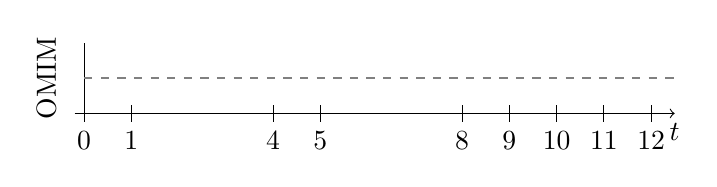
\begin{tikzpicture}[scale=0.6]
			\schedule{12.5}{OMIM}{1,4,5,8,9,10,11,12}
			\taskB{0}
			\taskC{1}
			\taskA[1]{5}
			\taskD[1]{8}
			\end{tikzpicture}
		}
		
		\subfloat[][Memory Capacity: 6]{
			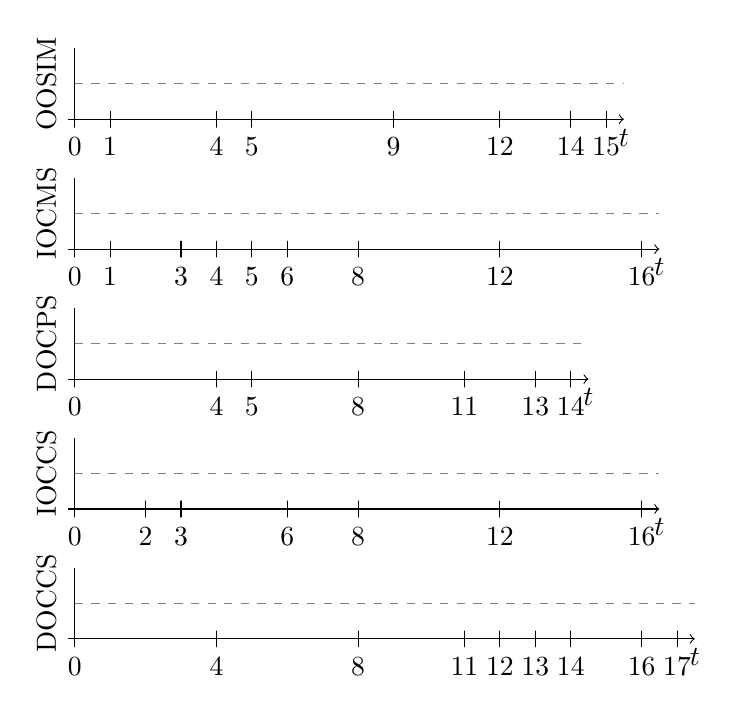
\begin{tikzpicture}[yscale=0.6, xscale=0.45]
			\begin{scope}
			\schedule{15.5}{OOSIM}{1,4,5,9,12,14,15}
			\taskB{0}
			\taskC{1}
			\taskA{9}
			\taskD{12}
			\end{scope}
			\begin{scope}[yshift=-2.75cm]
			\schedule{16.5}{IOCMS}{1,3,4,5,6,8,12,16}
			\taskB{0}
			\taskD[1]{1}
			\taskA{3}
			\taskC{8}
			\end{scope}
			\begin{scope}[yshift=-5.5cm]
			\schedule{14.5}{DOCPS}{4,5,8,11,13,14}
			\taskC{0}
			\taskB[3]{4}
			\taskA{8}
			\taskD{11}
			\end{scope}
			\begin{scope}[yshift=-8.25cm]
			\schedule{16.5}{IOCCS}{2,3,6,8,12,16}
			\taskD{0}
			\taskB{2}
			\taskA{3}
			\taskC{8}
			\end{scope}
			\begin{scope}[yshift=-11cm]
			\schedule{17.5}{DOCCS}{4,8,11,12,13,14,16,17}
			\taskC{0}
			\taskA{8}
			\taskB[1]{11}
			\taskD[2]{12}
			\end{scope}
			\end{tikzpicture}
		}
		
		\caption{ \label{fig:staticOrderExample} Static order heuristic schedules for Table~\ref{tab:staticOrderExample}.} 
		%%			Optimal schedule length	is 14. 
	\end{figure}
	
	%%\begin{figure}[htb]
	%%	
	%%	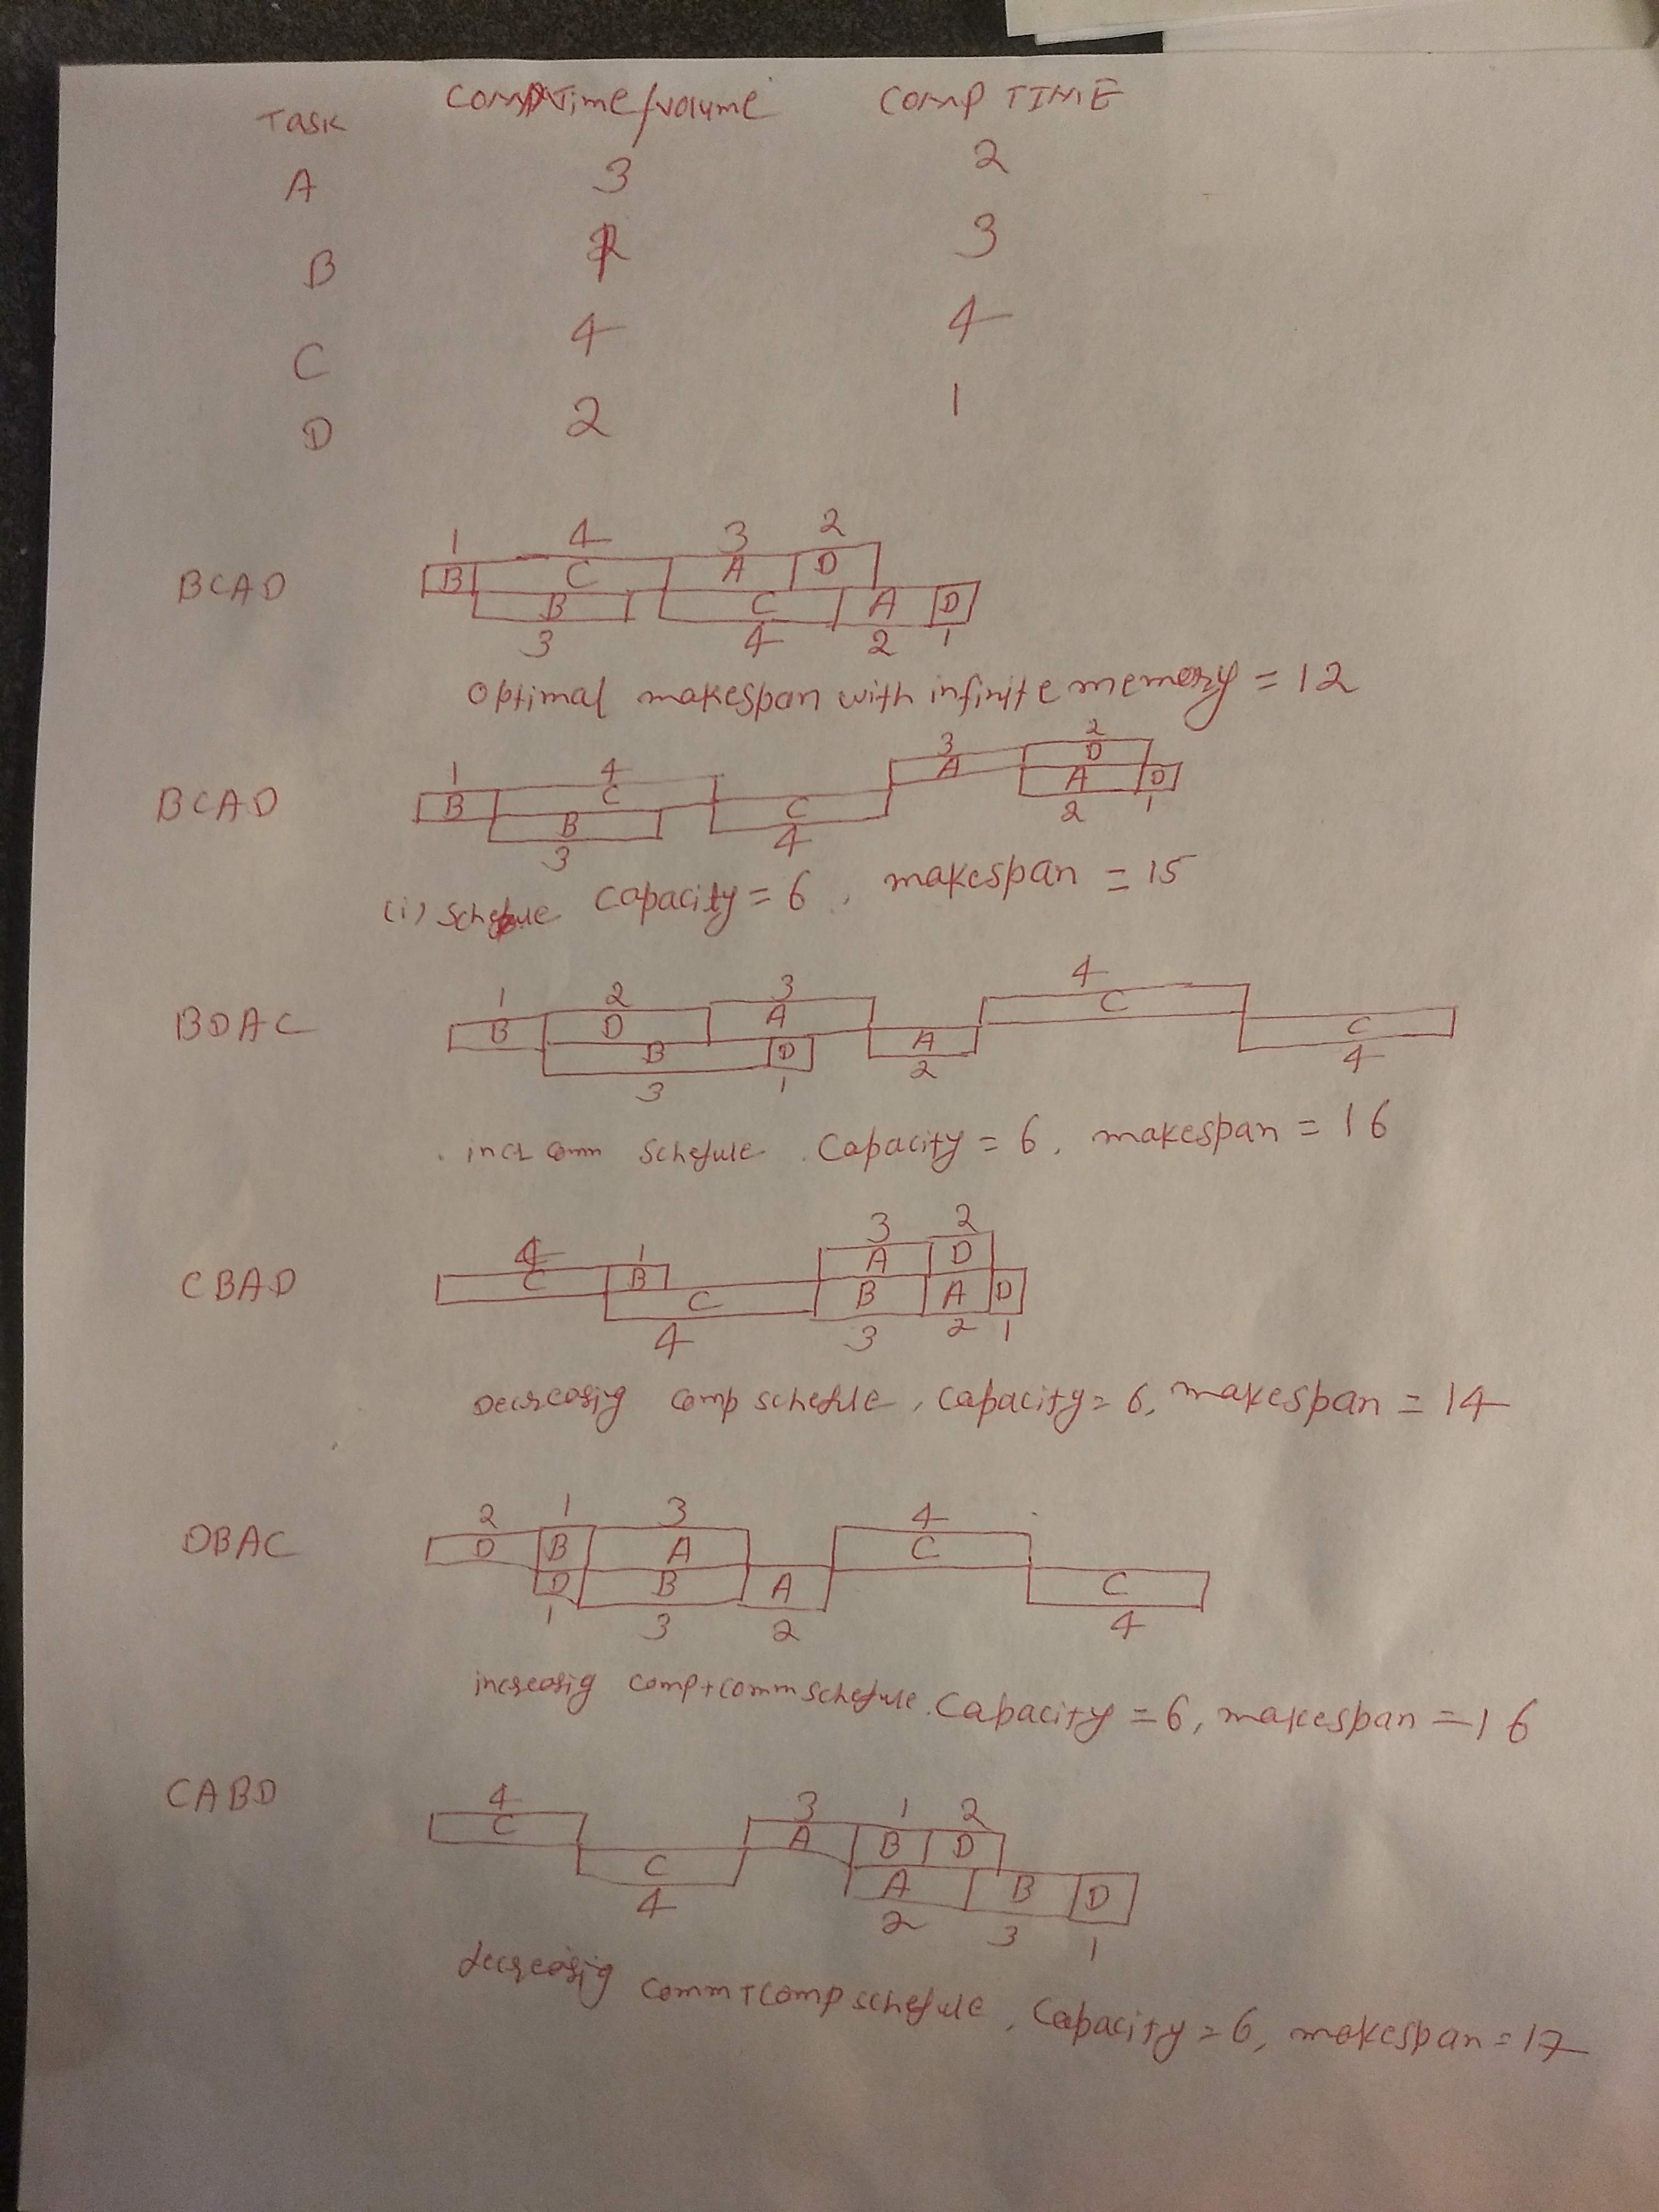
\includegraphics[scale=0.05]{Figs/staticOrderSchedules}
	%%			\caption{Task set and schedules where orders are precomputed based on different heuristics.}
	%%	\label{fig:staticOrderExample}
	%%\end{figure}
	
	In order to highlight the different behaviors of these static strategies, we propose on Table~\ref{tab:staticOrderExample} an example instance, and on Figure~\ref{fig:staticOrderExample} the corresponding schedules for all these heuristics.
	
	
	
	
	\subsection{Dynamic Selection}
	Dynamic strategies are based on the following principle: when the communication resource is idle, a task is chosen based on a selection criterion which differs depending on the heuristic, among those which fit in memory and induce minimum idle time on the computation resource.  For example, if the selection criterion is to choose a highly compute intensive task, then we compute the ratio of computation time and communication time for all tasks, and we select a task with the maximum ratio among those which induce minimum idle time on the computation resource and fit in the currently available memory. If no task fits in memory then we leave the resource idle at that point and proceed to the next event point. 
%%	We also ensure that the order on both resources is the same, by ordering tasks on the computation resource accordingly.
	
	%%	If $COMM_A = 1, COMP_A=1, COMM_B=2, COMP_B=4$, then $MAMR$ heuristic first selects task $A$ (A induces less idle tim eon the computation resource).  
	
	
	%%	\todo[inline]{LED: I added this part ``among those which fit in memory'', is it correct? SKumar: Yes, you are correct.}
	%%	\todo[inline]{LED: What happens if no task fit in memory? Skumar: look at the next event point :)}
	
	%% We select a set of tasks which induce minimum idle time on compute resource and satisfy available memory requirement. Then a task is chosen for processing from this set based on the following heuristics.
	\begin{enumerate}[label=\roman*)]
		\item \textit{largest communication task respects memory restriction} ($LCMR$): A task with the largest communication time is chosen. 
		\item \textit{smallest communication task respects memory restriction} ($SCMR$): A task with the smallest communication time is chosen.
		\item \textit{maximum accelerated task respects memory restriction} ($MAMR$): A task with the maximum ratio of computation time to communication time is chosen.
	\end{enumerate}
	\begin{table}[htb]
		\begin{center}
			
			\begin{tabular}{|c|c|c|c|}
				\hline
				%%				Task & Comm Volume & Comm Time & Comp Time\\ \hline 
				\multirow{2}{*}{Task} & Memory Req & \multirow{2}{*}{Comm Time} & \multirow{2}{*}{Comp Time}\\  
				&=Comm Volume && \\ \hline
				A & 3 & 3 & 2\\ \hline
				B & 1 & 1 &  6\\ \hline
				C & 4 & 4 & 6\\ \hline
				D & 5 & 5 & 1\\ \hline
			\end{tabular}
			\caption{\label{tab:dynamicSelectionExample} A task set for dynamic schedules.}
		\end{center}
	\end{table}
	
	\begin{figure}[htb]
		\centering
		
		\newcommand{\taskA}[2][0]{\task[#1]{$A$}{#2}{3}{2}{cyan}}
		\newcommand{\taskB}[2][0]{\task[#1]{$B$}{#2}{1}{6}{blue!40!white}}
		\newcommand{\taskC}[2][0]{\task[#1]{$C$}{#2}{4}{6}{blue!70!white}}
		\newcommand{\taskD}[2][0]{\task[#1]{$D$}{#2}{5}{1}{blue}}
		
		\centering
		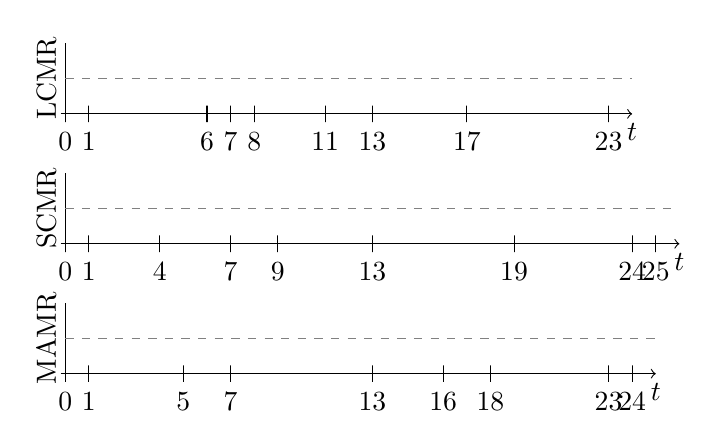
\begin{tikzpicture}[yscale=0.6,xscale=0.3]
		\begin{scope}
		\schedule{24}{LCMR}{1,6,7,8,11,13,17,23}
		\taskB{0}
		\taskD[1]{1}
		\taskA{8}
		\taskC{13}
		\end{scope}
		\begin{scope}[yshift=-2.75cm]
		\schedule{26}{SCMR}{1,4,7,9,13,19,24,25}
		\taskB{0}
		\taskA[3]{1}
		\taskC{9}
		\taskD{19}
		\end{scope}
		\begin{scope}[yshift=-5.5cm]
		\schedule{25}{MAMR}{1,5,7,13,16,18,23,24}
		\taskB{0}
		\taskC[2]{1}
		\taskA{13}
		\taskD{18}
		\end{scope}
		\end{tikzpicture}
		\caption{ \label{fig:dynamicSelectionExample} Different dynamic heuristic schedules for a task set of Table~\ref{tab:dynamicSelectionExample} with a memory capacity of 6.}
		%%		 Optimal schedule length is 23.
	\end{figure} 
	
	
	We highlight the different dynamic heuristics with the instance described on Table~\ref{tab:dynamicSelectionExample} (these heuristics are too similar on the instance from the previous class), and Figure~\ref{fig:dynamicSelectionExample} shows the corresponding schedules.
	
	\subsection{Static Order with Dynamic Corrections}
	
	In this class of strategy, we precompute the order of tasks based on some criterion and then follow this ordering as much as possible. But when the communication resource is idle because the memory requirement of the next task is too high, then we select a task  with a dynamic strategy. After a task is dynamically selected, we update the remaining order without this task. This class of strategy takes advantage of static information in the form of precomputed order and dynamic corrections to minimize the idle time due to memory constraint.
	
	In all strategies of this class, the initial order is $OMIM$ order,  obtained by Algorithm~\ref{alg:OrderOfExecutionInfinteMemory}. We define the following heuristics based on how we select a task from the set of tasks which fit in memory and induce minimum idle time on the computation resource. If no task fits in memory then we leave the resource idle and forward to the next event point.
	%%	\todo[inline]{LED: What happens if no task fit in memory?}
	
	\begin{enumerate}[label=\roman*)]
		\item \textit{optimal order infinite memory largest communication task respects memory restriction} ($OOLCMR$): A task with the largest communication time is chosen from the set.
		\item \textit{optimal order infinite memory smallest communication task respects memory restriction} ($OOSCMR$): A task with the smallest communication time is chosen from the set.
		\item \textit{optimal order infinite memory maximum accelerated task respects memory restriction} ($OOMAMR$): A task  with the maximum ratio of computation time to communication time is chosen from the set.
	\end{enumerate}
	
	\begin{table}[htb]
		\begin{center}
			
			\begin{tabular}{|c|c|c|c|}
				\hline
				%%				Task & Comm Volume & Comm Time & Comp Time\\ \hline 
				\multirow{2}{*}{Task} & Memory Req & \multirow{2}{*}{Comm Time} & \multirow{2}{*}{Comp Time}\\  
				&=Comm Volume && \\ \hline
				A & 4 & 4 &  1\\ \hline
				B & 2 & 2 & 6\\ \hline
				C & 8 & 8 & 8\\ \hline
				D & 5 & 5 & 4\\ \hline
				E & 3 & 3 & 2\\ \hline
			\end{tabular}
			\caption{\label{tab:staticOrderDynamicCorrectionsExample} A task set for static order dynamic corrections schedules.}
		\end{center}
	\end{table}
	
	\begin{figure}[htb]
		\newcommand{\taskA}[2][0]{\task[#1]{$A$}{#2}{4}{1}{cyan}}
		\newcommand{\taskB}[2][0]{\task[#1]{$B$}{#2}{2}{6}{cyan!50!black}}
		\newcommand{\taskC}[2][0]{\task[#1]{$C$}{#2}{8}{8}{blue!40!white}}
		\newcommand{\taskD}[2][0]{\task[#1]{$D$}{#2}{5}{4}{blue!70!white}}
		\newcommand{\taskE}[2][0]{\task[#1]{$E$}{#2}{3}{2}{blue}}
		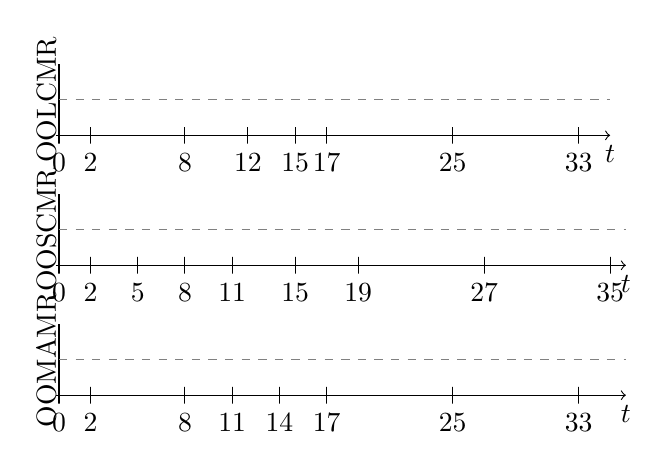
\begin{tikzpicture}[yscale=0.6,xscale=0.2]
		\begin{scope}
		\schedule{35}{OOLCMR}{2,8,12,15,17,25,33}
		\taskB{0}
		\taskD[1]{2}
		\taskA{8}
		\taskE{12}
		\taskC{17}
		\end{scope}
		\begin{scope}[yshift=-2.75cm]
		%%		\schedule{36}{OOSCMR}{2,5,8,11,14,18,26,34}
		%%		\taskB{0}
		%%		\taskE[3]{2}
		%%		\taskA[1]{5}
		%%		\taskD{9}
		%%		\taskC{18}
		%%		\end{scope}
		\schedule{36}{OOSCMR}{2,5,8,11,15,19,27,35}
		\taskB{0}
		\taskE[3]{2}
		\taskA[1]{5}
		\taskD{10}
		\taskC{19}
		\end{scope}
		\begin{scope}[yshift=-5.5cm]
		\schedule{36}{OOMAMR}{2,8,11,14,17,25,33}
		\taskB{0}
		\taskD[1]{2}
		\taskE[1]{8}
		\taskA{12}
		\taskC{17}
		\end{scope}
		%%		\begin{scope}[yshift=+2.75cm]
		%%		\schedule{40}{OMIM}{2,8,16,24,29,33,38}
		%%		\taskB{0}
		%%		\taskC{8}
		%%		\taskD{24}
		%%		\taskA{29}
		%%		\taskE{33}
		%%		\end{scope}
		
		\end{tikzpicture}
		\caption{ \label{fig:staticOrderDynamicCorrectionsExample} Different static order dynamic corrections heuristic schedules for a task set of Table~\ref{tab:staticOrderDynamicCorrectionsExample} with a memory capacity of 9. The $OMIM$ order is $BCDAE$.}
	\end{figure} 
	
	
	%%\begin{figure}[htb]
	%%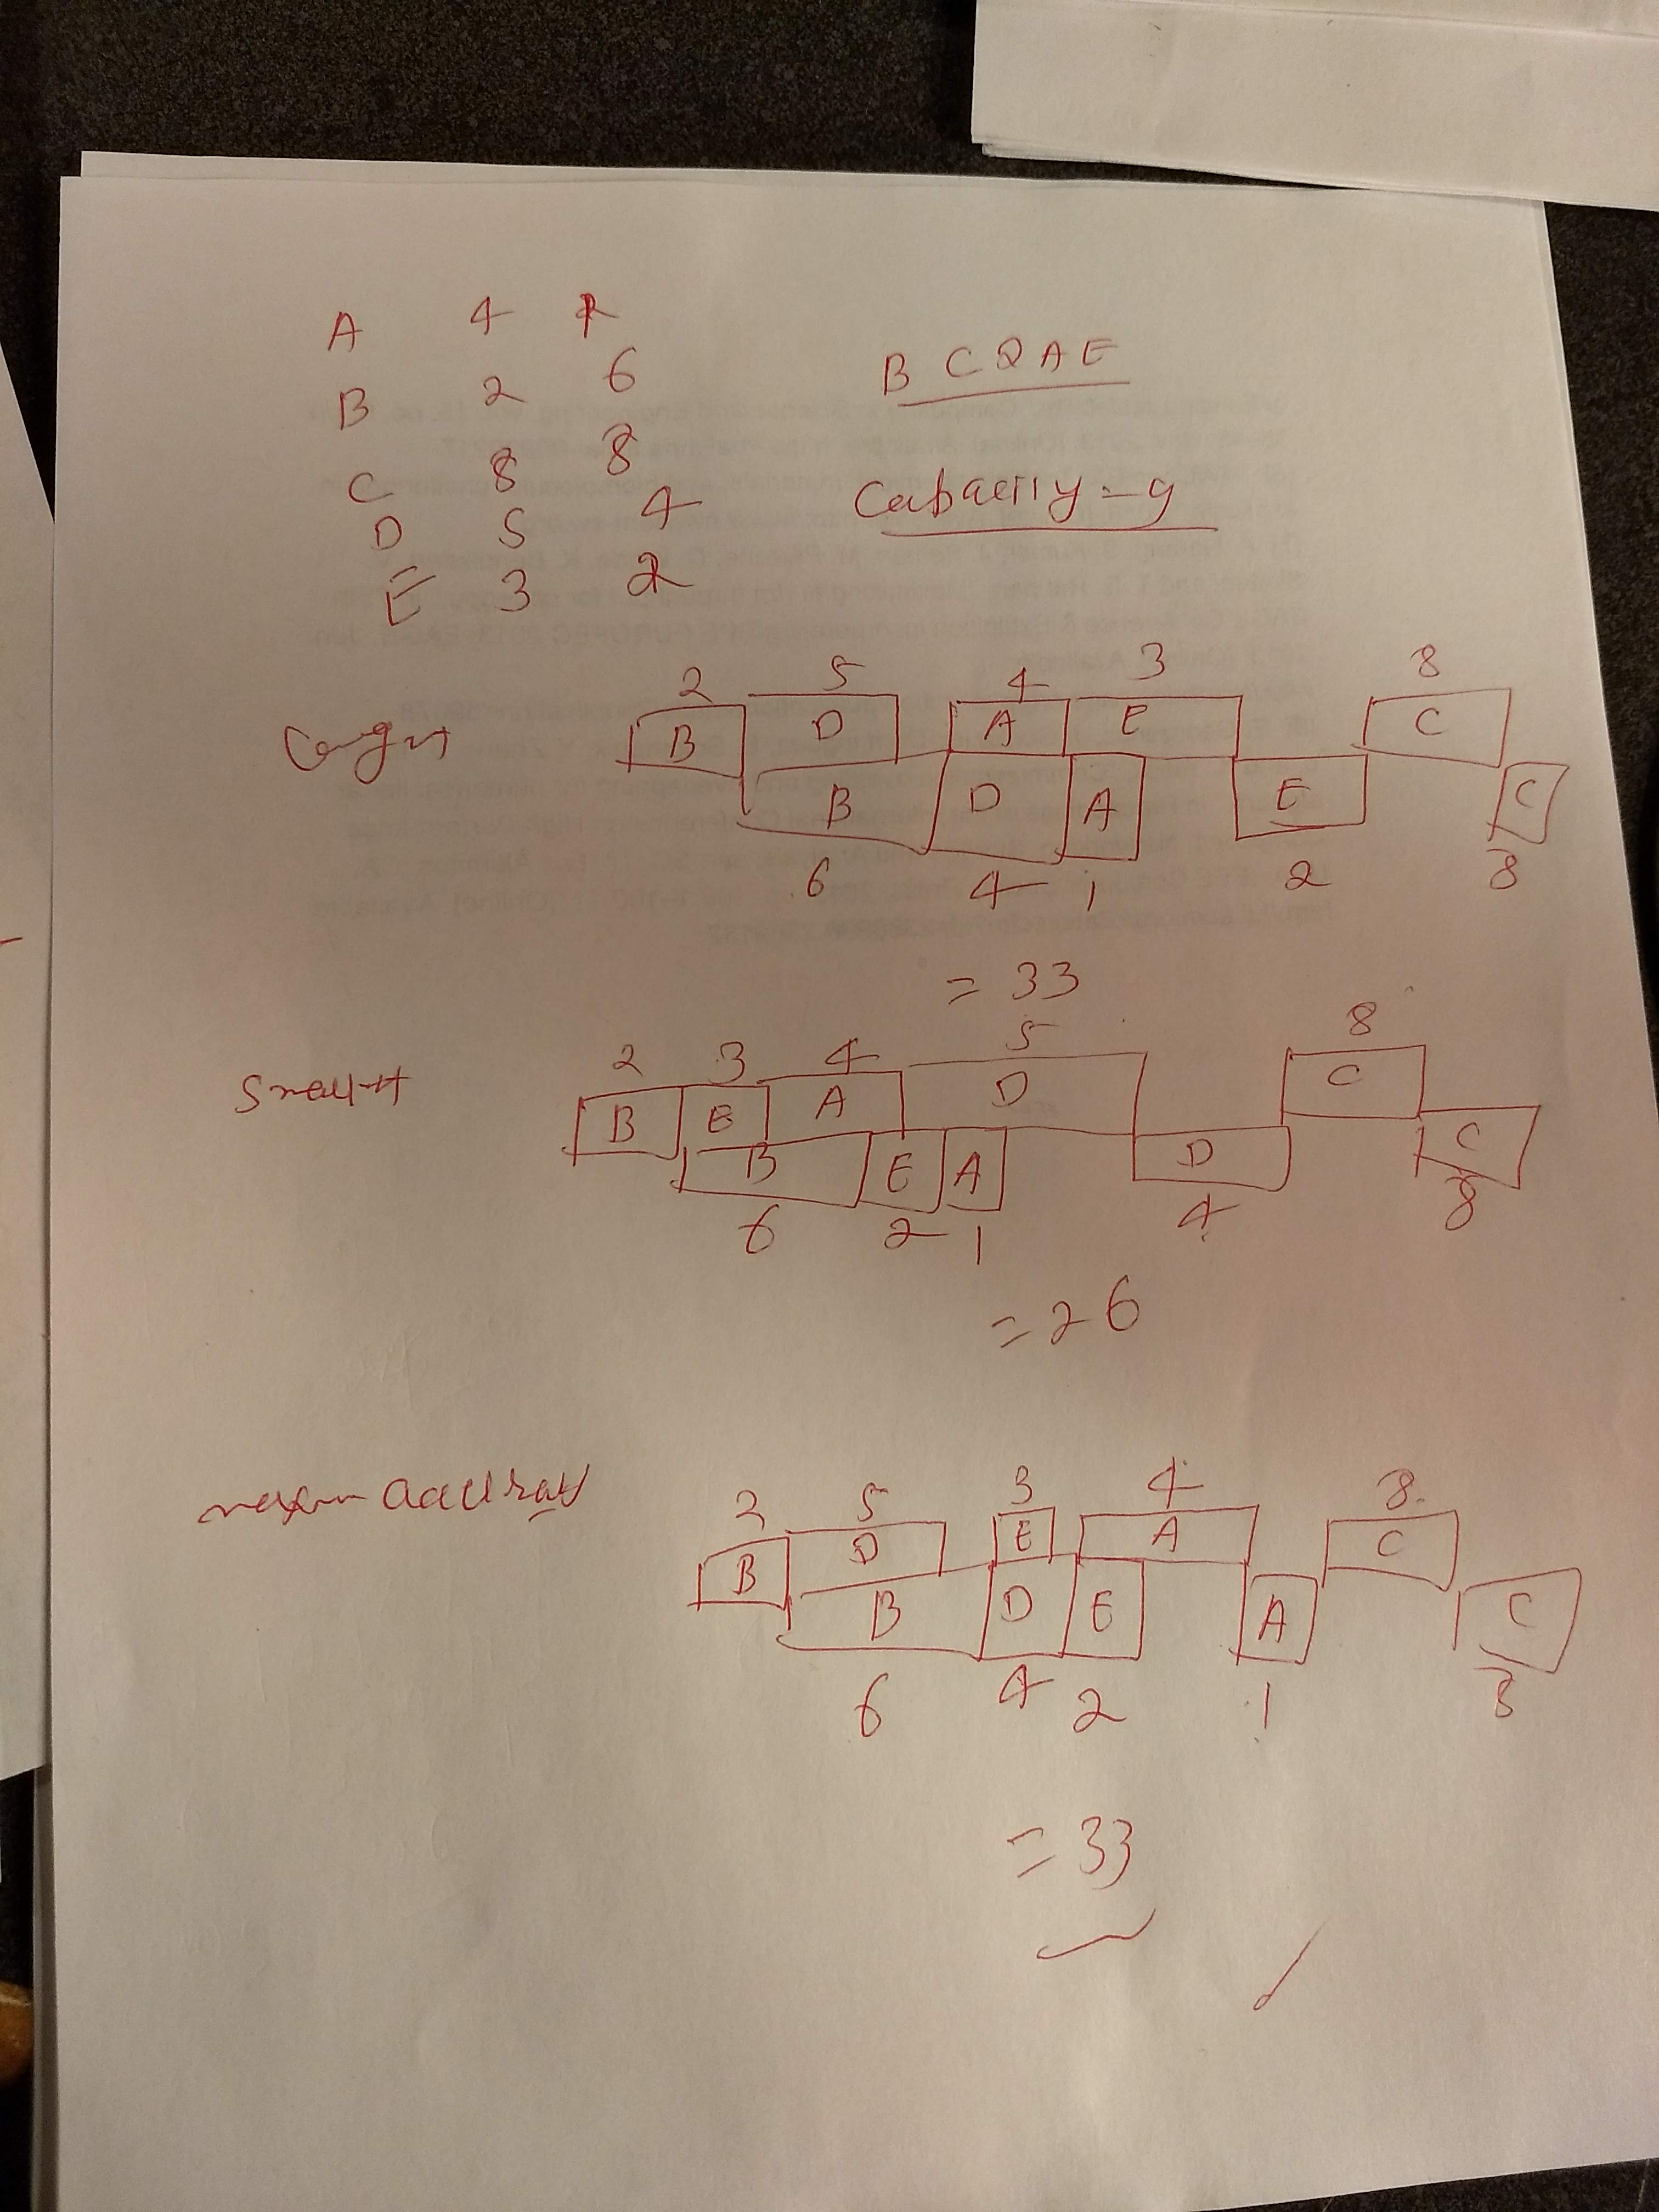
\includegraphics[scale=0.05]{Figs/staticOrderDynamicCorrectionsSchedules}
	%%\caption{Task set and schedules where orders are precomputed based on different heuristics.}
	%%\label{fig:staticOrderDynamicCorrectionsExample}
	%%\end{figure}
	
	As previously, we propose on Table~\ref{tab:staticOrderDynamicCorrectionsExample} an example instance for this class of strategies, and provide on Figure~\ref{fig:staticOrderDynamicCorrectionsExample} the corresponding schedules.
	
	\subsection{Additional Heuristics from Previous Work}
	
	We also consider two other static heuristics for evaluation. The first heuristic is based on an algorithm, proposed by Gilmore and Gomory, to obtain the minimal cost sequence for a set of jobs~\cite{Gilmore-Gomory:1964}. This is a classical algorithm for 2-machine no-wait flow shop. In this algorithm, each job has a start and end state and a cost is associated to change the state. In our context, this cost can be seen as non-overlap time of computation for two adjacent tasks. Here is the main idea of this algorithm. Initially, a partial sequence of jobs is represented by a graph such that their overlap is maximum. Subsequently edges are greedily added to this graph to connect two components while minimizing the total non-overlap cost. When the graph is  connected, an edge interchange mechanism is used to determine the sequence of jobs, which ensures that the sequence has minimal cost. More details can be found in the original paper~\cite{Gilmore-Gomory:1964} and our implementation is publicly available~\cite{gitworkrepo}. This algorithm does not take memory constraints into account and only provides the sequence of processing. We use this sequence with a memory capacity restriction just like for other static heuristcs, and we call this heuristic \textit{Gilmore-Gomory} ($GG$).
	
	The second heuristic is based on the First-Fit algorithm for the bin packing problem. The idea of this heuristic is to identify groups of tasks which can fit in memory together, called \emph{bins}. In First-Fit, tasks are considered in an arbitrary order and added to the first bin in which they can fit. If no suitable bin is found then a new bin is created and this task is added to it. When all tasks have been assigned to bins, we consider the sequence made of all tasks from the first bin, then tasks for the second bin, and so on. We call this heuristic \textit{Bin Packing} ($BP$). 
	
	
	\subsection{Solving Linear Program Iteratively}
	\label{subsec:linearprogrammingformulation}
	We use a mixed integer linear program to obtain the order of communications and computations. Recall that $COMP_i$ and $COMM_i$ represent computation and communication times of task $i$, and the memory capacity of the target system is $C$. In the linear program formulation, $s_i$ and $e_i$ (resp. $s'_i$ and $e'_i$) represent the start and end times of communication (resp. computation) for task $i$, and $MC(i)$ is the memory capacity requirement of task $i$. The formulation also contains for each pair of tasks $i$ and $j$ \textit{i)} a boolean variable $a_{ij}$ to denote the order of $i$ and $j$ on the communication resource \textit{ii)} a boolean variables $b_{ij}$ to denote the order of $i$ and $j$ on the computation resource, and \textit{iii)} a boolean variables $c_{ij}$ to denote the order of $s_i$ and $e'_j$. 
	
	
	%% $TM(i)$ denotes intermediate memory requirement of task $T_i$ . 
	
	%%, and $iv)$ (optional, if we consider temporary buffer requirement for each task) n-1 boolean variables, $d_{ij}$, for each task $T_i$ to denote the order of $e'_i$ and $s_j$.
	
	
	
	\noindent Let $L=\sum_i (COMP_i + COMM_i)$. It is evident that $e_i =s_i + COMM_i$ and $e'_i =s'_i + COMP_i$. The linear program is given below.
	
	\vspace*{-0.5cm}
	\begin{align*}
		& \text{Minimize $l$ subject to:}\\
		\forall i, \quad & e'_i \leq l && \text{(task $i$ completes)}\\
		\forall i, \quad & e_i \leq s'_i&& \text{(task $i$ valid ordering)}\\
		\forall i, \forall j\ne i, \quad & \left\{\begin{aligned}
			e_j & \leq s_i +(1-a_{ij})L\\
			e_i & \leq s_j +a_{ij}L 
		\end{aligned} \right. &&
		\begin{aligned}
			&\text{(exclusive use of}\\
			&\text{  communication link)}
		\end{aligned}\\
		\forall i, \forall j\ne i, \quad & \left\{
		\begin{aligned}
			e'_j &\leq s'_i +(1-b_{ij})L\\
			e'_i &\leq s'_j +b_{ij}L
		\end{aligned}\right. && 
		\begin{aligned}
			&\text{(exclusive use of}\\
			&\text{  computation resource)}
		\end{aligned}\\
		\forall i, \forall j\ne i, \quad &\left\{
		\begin{aligned}
			e'_j &\leq s_i +(1-c_{ij})L\\
			s_i  &< e'_j +c_{ij}L\\
		\end{aligned}\right.&&
		\begin{aligned}
			&\text{(respect ordering}\\
			&\text{ of variables $c_{ij}$)}
		\end{aligned}\\
		\forall i, \quad & \sum_{r\ne i} (a_{ir} - c_{ir})MC(r) + MC(i) \le C && \text{(memory constraint)}\\
		%% %%\forall i, \forall j\ne i, \quad & \text{task }T_i \text{ respects memory capacity on computation resource:}\\
		%% %%& s_j < e'_i +(1-d_{ij})L\\
		%% %%& e'_i\leq s_j +d_{ij}L\\
		%% %%& \sum_r (d_{ir} - b_{ir})CM(r) + TM(i) \le C\\
	\end{align*} 
	
	
	We use GLPK solver v4.65 to solve the above formulation. We also add the following constraints to help the solver: $\forall i, \forall j\ne i$, $a_{ij} + a_{ji}=1$, $b_{ij} + b_{ji} = 1$, $c_{ij} \le a_{ij}$, $c_{ij} \le b_{ij}$, and  $c_{ij} + c_{ji} \le 1$. The solver was unable to  solve this MILP at the scale of our interest in limited time. Hence, we solve the linear program iteratively for a small subset of size $k=3, 4, 5, 6$: at the boundary of two iterations we fix the event (communication or computation) of an unfinished task started before the boundary point and consider other events flexible. The subsets are formed in the order in which tasks are submitted, which is arbitrary. For a given size $k$, we represent the makespan calculated by this heuristic as $lp.k$.
	We compute various $lp.k$ values for different memory capacities and observe that most of the other heuristics perform better than this heuristic. Hence, we do not include this heuristic for the comparison in Section~{\ref{sec:expResults}. Performance comparison of different heuristics with MILP based heuristics is available in an extended version~\cite{extendedVersion}.
		
		%%		\todo[inline]{SKumar: Move to an extended version and more clear about results and implementation}
		%%		Figure~\ref{fig:iterativeLpSolution} shows the performance of different heuristics with MILP based heuristics for various memory capacities of a single trace file.
		%%		%%	\subsection{MILP Based Strategy}
		%%		%%We use GLPK solver v4.65 to solve the MILP formulation described in Section~\ref{subsec:linearprogrammingformulation}. The solver was unable to handle number of variables required to solve MILP at the scale of our interest. Hence, we solve the linear program iteratively for a small subset of size $k=3,4,5$ (solver was unable to handle number of variables required for $k\ge6$ ) and represent the makespan calculated by this heuristic as $lp.k$. At the boundary of two iterations we fixed the event (communication or computation) of an unfinished task who has started before the boundary point and consider other events flexible. We compute various $lp.k$ values for different memory capacities and observe that most of the other heuristics perform better than this heuristic. Figure~\ref{fig:iterativeLpSolution} shows the comparison of different heuristics with MILP based heuristic for various memory capacities of a single trace file.
		%%		\todo[inline]{SKumar: Figure~\ref{fig:iterativeLpSolution} would be removed and I will redraw this or similar figure for extended version}
		%%		\begin{figure}[htb]
		%%			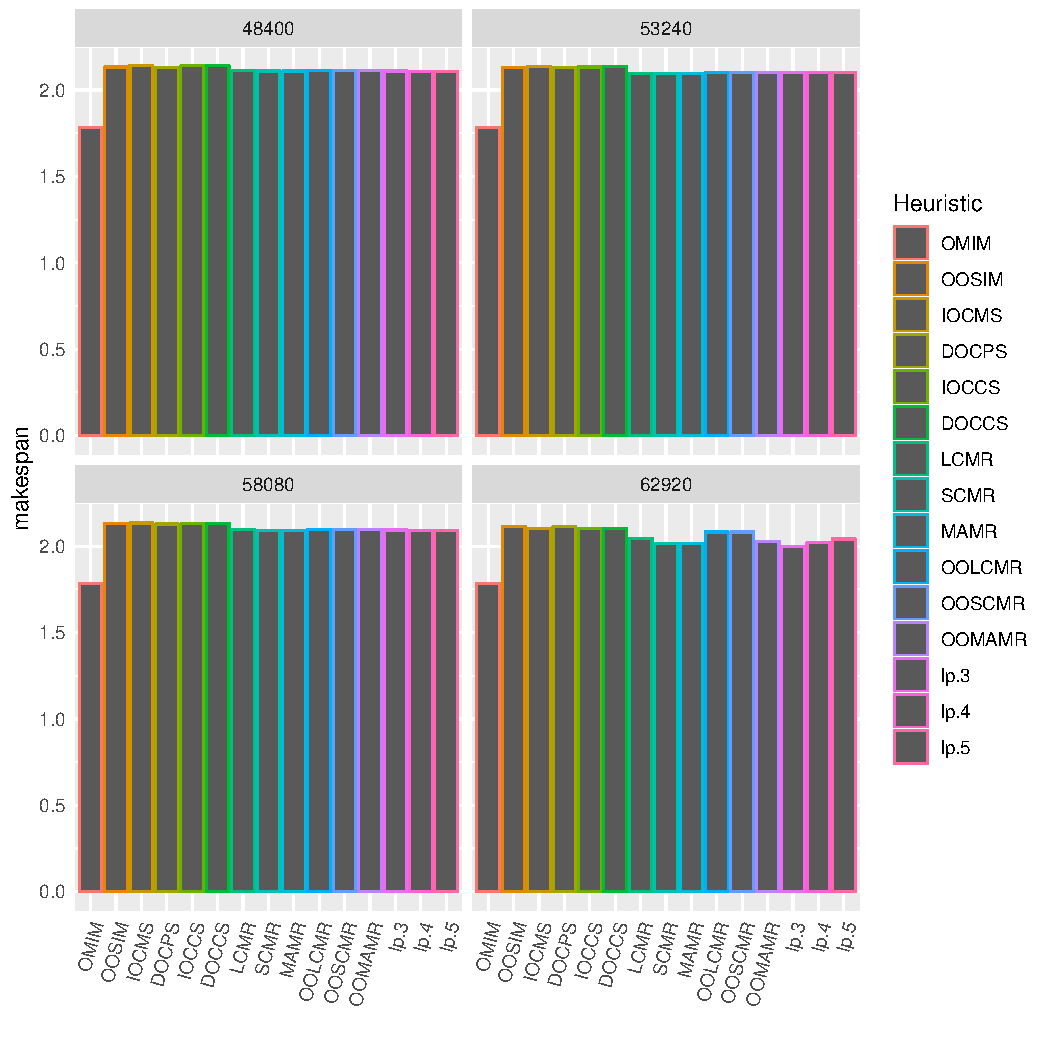
\includegraphics[scale=0.5]{./results/makespan_with_lp.pdf}
		%%			\caption{Comparison of different heuristics with MILP solution based heuristic.\todo[inline]{LED: I understand that this figure will be removed? Otherwise, use aes(fill=) instead of aes(color=) to have color filled bars.}}
		%%			\label{fig:iterativeLpSolution}
		%%		\end{figure}
		
		\subsection{Favorable Situations for Heuristics}
		Based on the definition of proposed strategies and the optimality of Algorithm~\ref{alg:OrderOfExecutionInfinteMemory}, we present the scenarios which should be more favorable for each heuristic in Table~\ref{tab:heuristicsAndFavorableScenarios}. This allows programmers to use appropriate strategies to maximize communication-computation overlap for their applications. In this table, ``moderate memory capacity'' refers to the case where memory is constrained, but close to the maximal memory requirement of the $OMIM$ schedule.
		
		\begin{table}[htb]
			\begin{tabular}{|c|p{6.5cm}|}
				\hline
				\textbf{Heuristic} & \textbf{\hspace{2cm}Favorable Situation} \\ \hline
				$OOSIM$ & Memory capacity is not a restriction (\textcolor{green}{Optimal}) \\ \hline
				$IOCMS$ & Memory capacity is not a restriction and tasks are compute intensive (\textcolor{green}{Optimal}) \\ \hline
				$DOCPS$ & Memory capacity is not a restriction and tasks are communication intensive (\textcolor{green}{Optimal}) \\ \hline
				$IOCCS$ & Moderate memory capacity and most tasks are highly compute intensive \\ \hline
				$DOCCS$ & Moderate memory capacity and most tasks are highly communication intensive \\ \hline
				$LCMR$ & Limited memory capacity and significant percentage of tasks with large communication times are compute intensive\\ \hline
				$SCMR$ & Limited memory capacity and significant percentage of tasks with small communication times are compute intensive\\ \hline
				$MAMR$ & Limited memory capacity and significant percentage of all types of tasks\\ \hline
				$OOLCMR$ & Moderate memory capacity and significant percentage of slightly communication intensive tasks have large communication times\\ \hline
				$OOSCMR$ & Moderate memory capacity and significant percentage of slightly communication intensive tasks have small communication times\\ \hline
				$OOMAMR$ & Moderate memory capacity and significant percentage of all types of tasks \\ \hline
			\end{tabular}\caption{~\label{tab:heuristicsAndFavorableScenarios}Heuristics and their favorable scenarios.}
		\end{table}
		
		Some of these favorable scenarios can be clearly observed in our experimental results, on Figures~\ref{fig:ratio_to_optimal_hf} and~\ref{fig:ratio_to_optimal_ccsd}. For example, HF compute intensive tasks have small communication times, which explains why the $SCMR$ heuristic exhibits very good performance in limited memory cases. CCSD has significant percentage of large as well as small types of slightly communication intensive tasks, and indeed the performance of $OOLCMR$ and $OOSCMR$ is very close to optimality in moderate memory cases. 
		%%		\todo[inline]{Skumar: Initially I placed this table after results. Then I realized that this is our hypothesis not conclusion. Only few favorable scenarios are matched with results. We do not have enough results to show favorable scenarios for all of them.}
		%%		\todo[inline]{LED: Ok. I did a rephrasing there to go in this direction, make sure it fits the message you wanted to say.}
		
		\section{Experimental Settings}
		\label{sec:expSetting}
		
		We consider a machine called Cascade~\cite{Cascade}, available at PNNL, for our experiments. We obtain traces by running two molecular chemistry applications, double precision version of  HF and CCSD of NWChem~\cite{NWChem} package on 10 nodes of this machine. Each node is composed of 16 Intel Xeon E5-2670 cores. NWChem takes advantages of a Partitioned Global Address Space Programming Model called Global Arrays (GA)~\cite{GlobalArray} to use shared-memory programming APIs on distributed memory computers. GA dedicates one core of each node to handle other cores, hence we can view a node as being composed of 15 computational cores. We use 150 processes for each application and obtain 150 trace files. We run CCSD with Uracil molecules input and HF with SiOSi molecules (for Uracil molecules, HF has a much smaller workload, each processor executes only around 20 tasks, that is why we chose SiOSi input for HF execution). Each process executes around 300-800 tasks. Our data transfer model is quite simple and we consider that all data transfers between the local memory of each process and the GA memory take the same route. Modeling of different routes of data transfers for the same source-destination pair, bandwidth sharing for different source-destination pairs and network congestion is more challenging and part of our future work. This simple model is enough to provide insight to the application developers (or runtime system) about the ordering of data transfers for the same source-destination pair so as to maximize communication-computation overlap. Our model is easily adaptable to any source-destination pair when there is one fixed route between source and destination (such as between CPU and GPU, one copy engine to transfer data from CPU (resp. GPU) to GPU (resp. CPU) ).
		
		%%		\todo[inline]{More about tiling}
		Both applications mainly perform two types of computations, tensor transpose and tensor contraction. HF expects to specify a tile size and we set it to 100, so that each core can be used efficiently. CCSD automatically determines tile sizes at different program points based on the input molecules. Hence, HF operates on almost homogeneous tiles while CCSD uses more heterogeneous tiles.
		
		\subsection{Workload Characteristics}
		
		\begin{figure}[htb]
			%\begin{tabular}{c}
			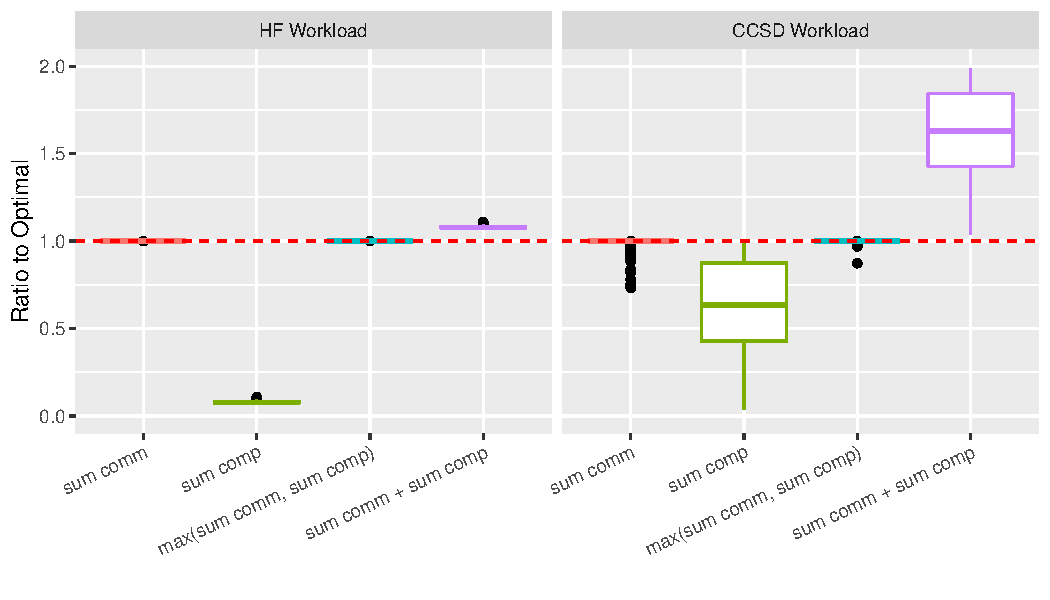
\includegraphics[scale=0.48]{./results/application_properties.pdf}
			\caption{HF and CCSD tasks characteristics.}
			\label{fig:ApplicationProperties}
		\end{figure}	
		
		To get more insights into the considered workloads, we provide  information about the instances we consider in Figure~\ref{fig:ApplicationProperties}. For each instance, we compute the sum of communication times (\textit{sum comm}) and sum of computation times  (\textit{sum comp}), and normalize it relatively to the $OMIM$ value. Figure~\ref{fig:ApplicationProperties} also shows the maximum of both values, which is a lower bound on the possible makespan of a schedule for this instance, and their sum, which is an upper bound: this represents the makespan of the sequential schedule, obtained with zero overlap between computation and communication. We can see that HF is a communication intensive application and at most 20\% overlap can be expected in the best scenario. On the other hand, in the CCSD workload, communications and computations are almost evenly distributed and a more significant overlap is possible.
		
		
		\section{Experimental Results}
		\label{sec:expResults}
		We evaluate our scheduling heuristics for several memory capacities. From the obtained traces, we first determine the minimum requirement of the memory capacity $m_c$ to execute all tasks. Then we observe the behavior of all heuristics with memory capacity $m_c$ to $2m_c$, in increments of $0.125m_c$. Our performance metric is the ratio to optimal $r$: if heuristic $H$ has makespan $M_H$ on an instance, and the optimal makespan for the infinite memory case is $OMIM$, then $r(H)=\frac{M_H}{OMIM}$ (lower values are better). This ratio is at least $1$, and a value close to $1$ indicates a well-suited  heuristic which achives maximum possible communication-computation overlap.
		
		Figures ~\ref{fig:ratio_to_optimal_hf} and ~\ref{fig:ratio_to_optimal_ccsd} show the distribution of the performance of each heuristic for different memory capacities, where plots are categorized by memory capacities. For each memory capacity and each heuristic, the box on the plot displays the median, first and last quartile, and the whiskers indicate minimum and maximum values, with outliers are shown by black dots.
		\subsection{HF Performance}	
		\begin{figure*}[htb]
			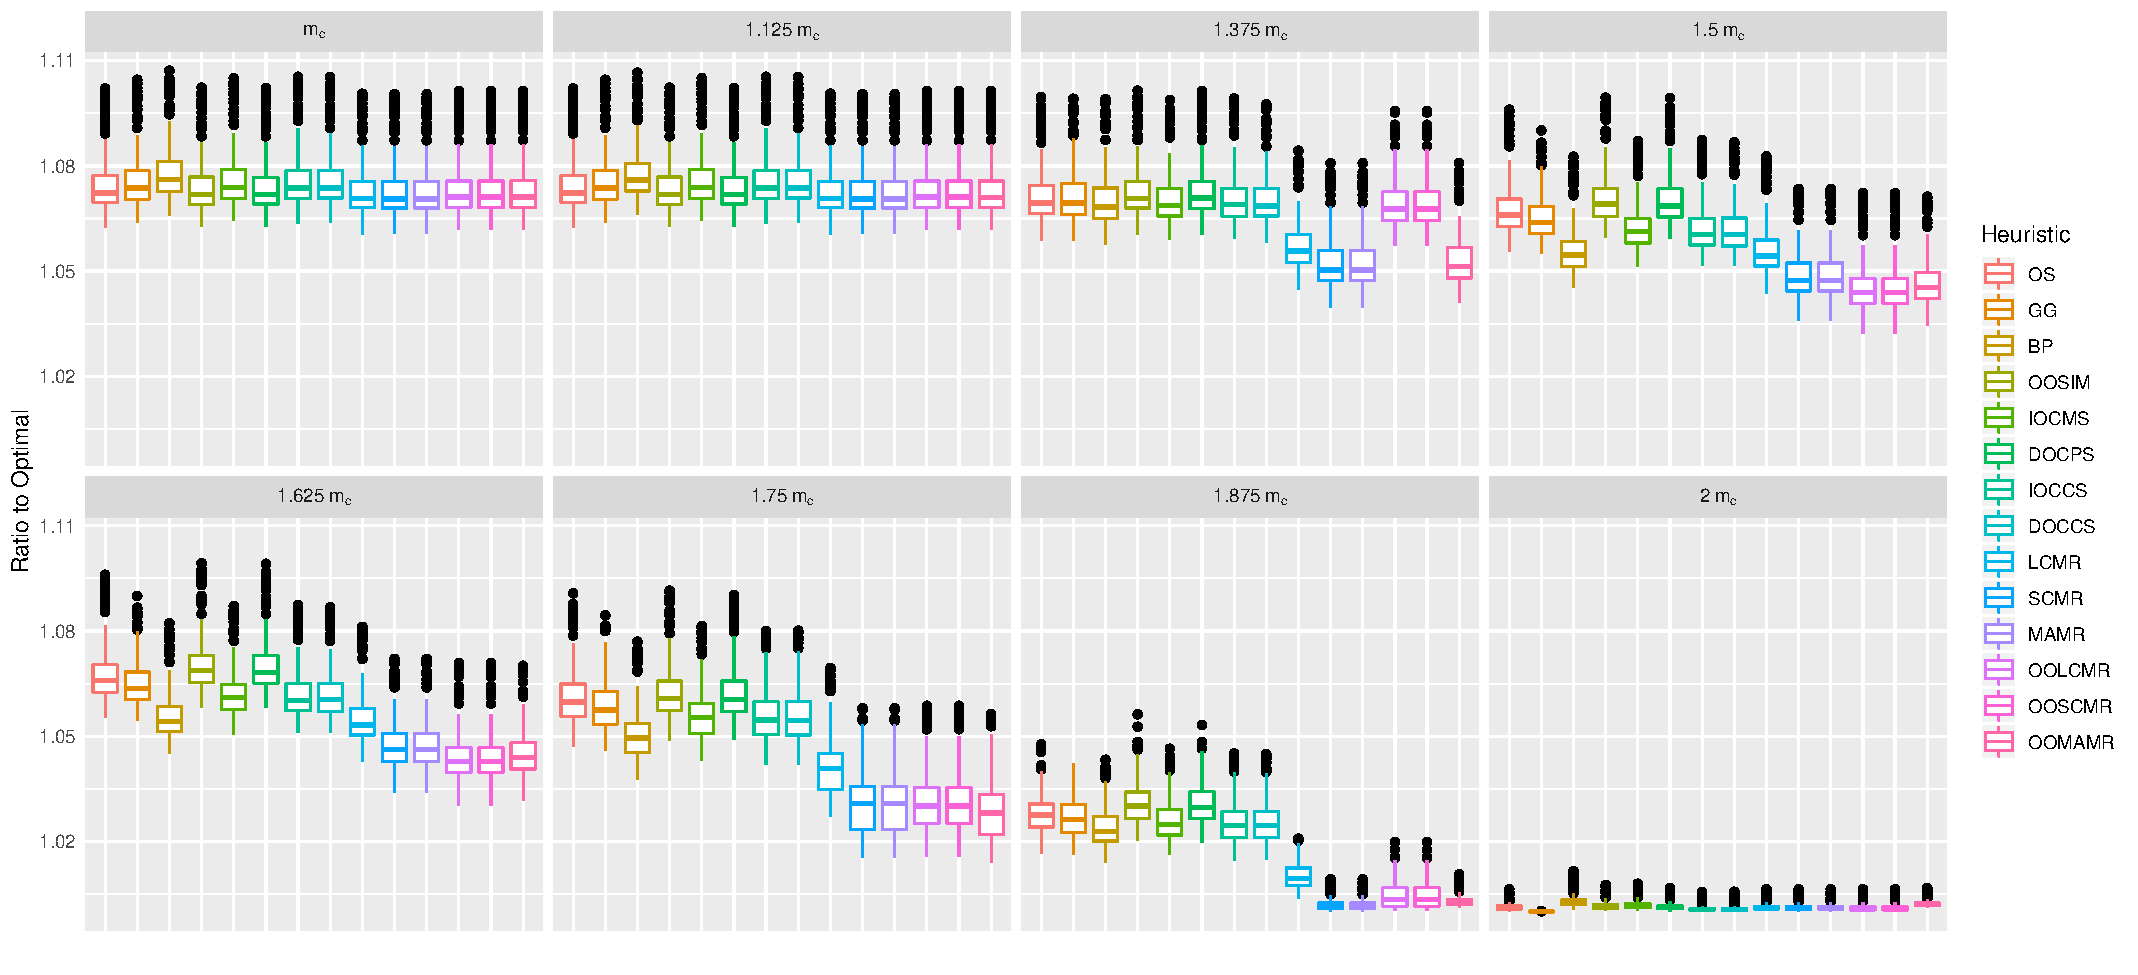
\includegraphics[scale=0.5]{./results/ratio_to_optimal_selected_hf.pdf}
			\caption{Comparison of different heuristics for HF with $m_c=176KB$.}
			\label{fig:ratio_to_optimal_hf}
		\end{figure*}
		
		As indicated above, HF tasks operate on less heterogeneous tiles, this is also noticeable in Figure~\ref{fig:ratio_to_optimal_hf}. All heuristics depict similar behavior for minimum memory capacity $m_c$ and increasing the memory capacity slightly does not change the performance of all heuristics. As memory capacity is increased further, dynamic variants of heuristics start performing better. For the moderate memory capacities (close to $2m_c$), static order with dynamic corrections variants outperform others. $GG$ heuristic does not achieve good performance, because its task sequence is obtained considering no extra memory is available, but is then applied in a different scenario where memory is limited. Surprisingly, the $BP$ heuristic which considers only memory constraint obtains good performance for a static heuristic, but is outperformed by more dynamic approaches.
		%%		\todo{you mean infinite memory? SKumar: GG is classic in no-wait (or no buffer) 2-macine flowshop}
		
		\begin{figure}[htb]
			%%			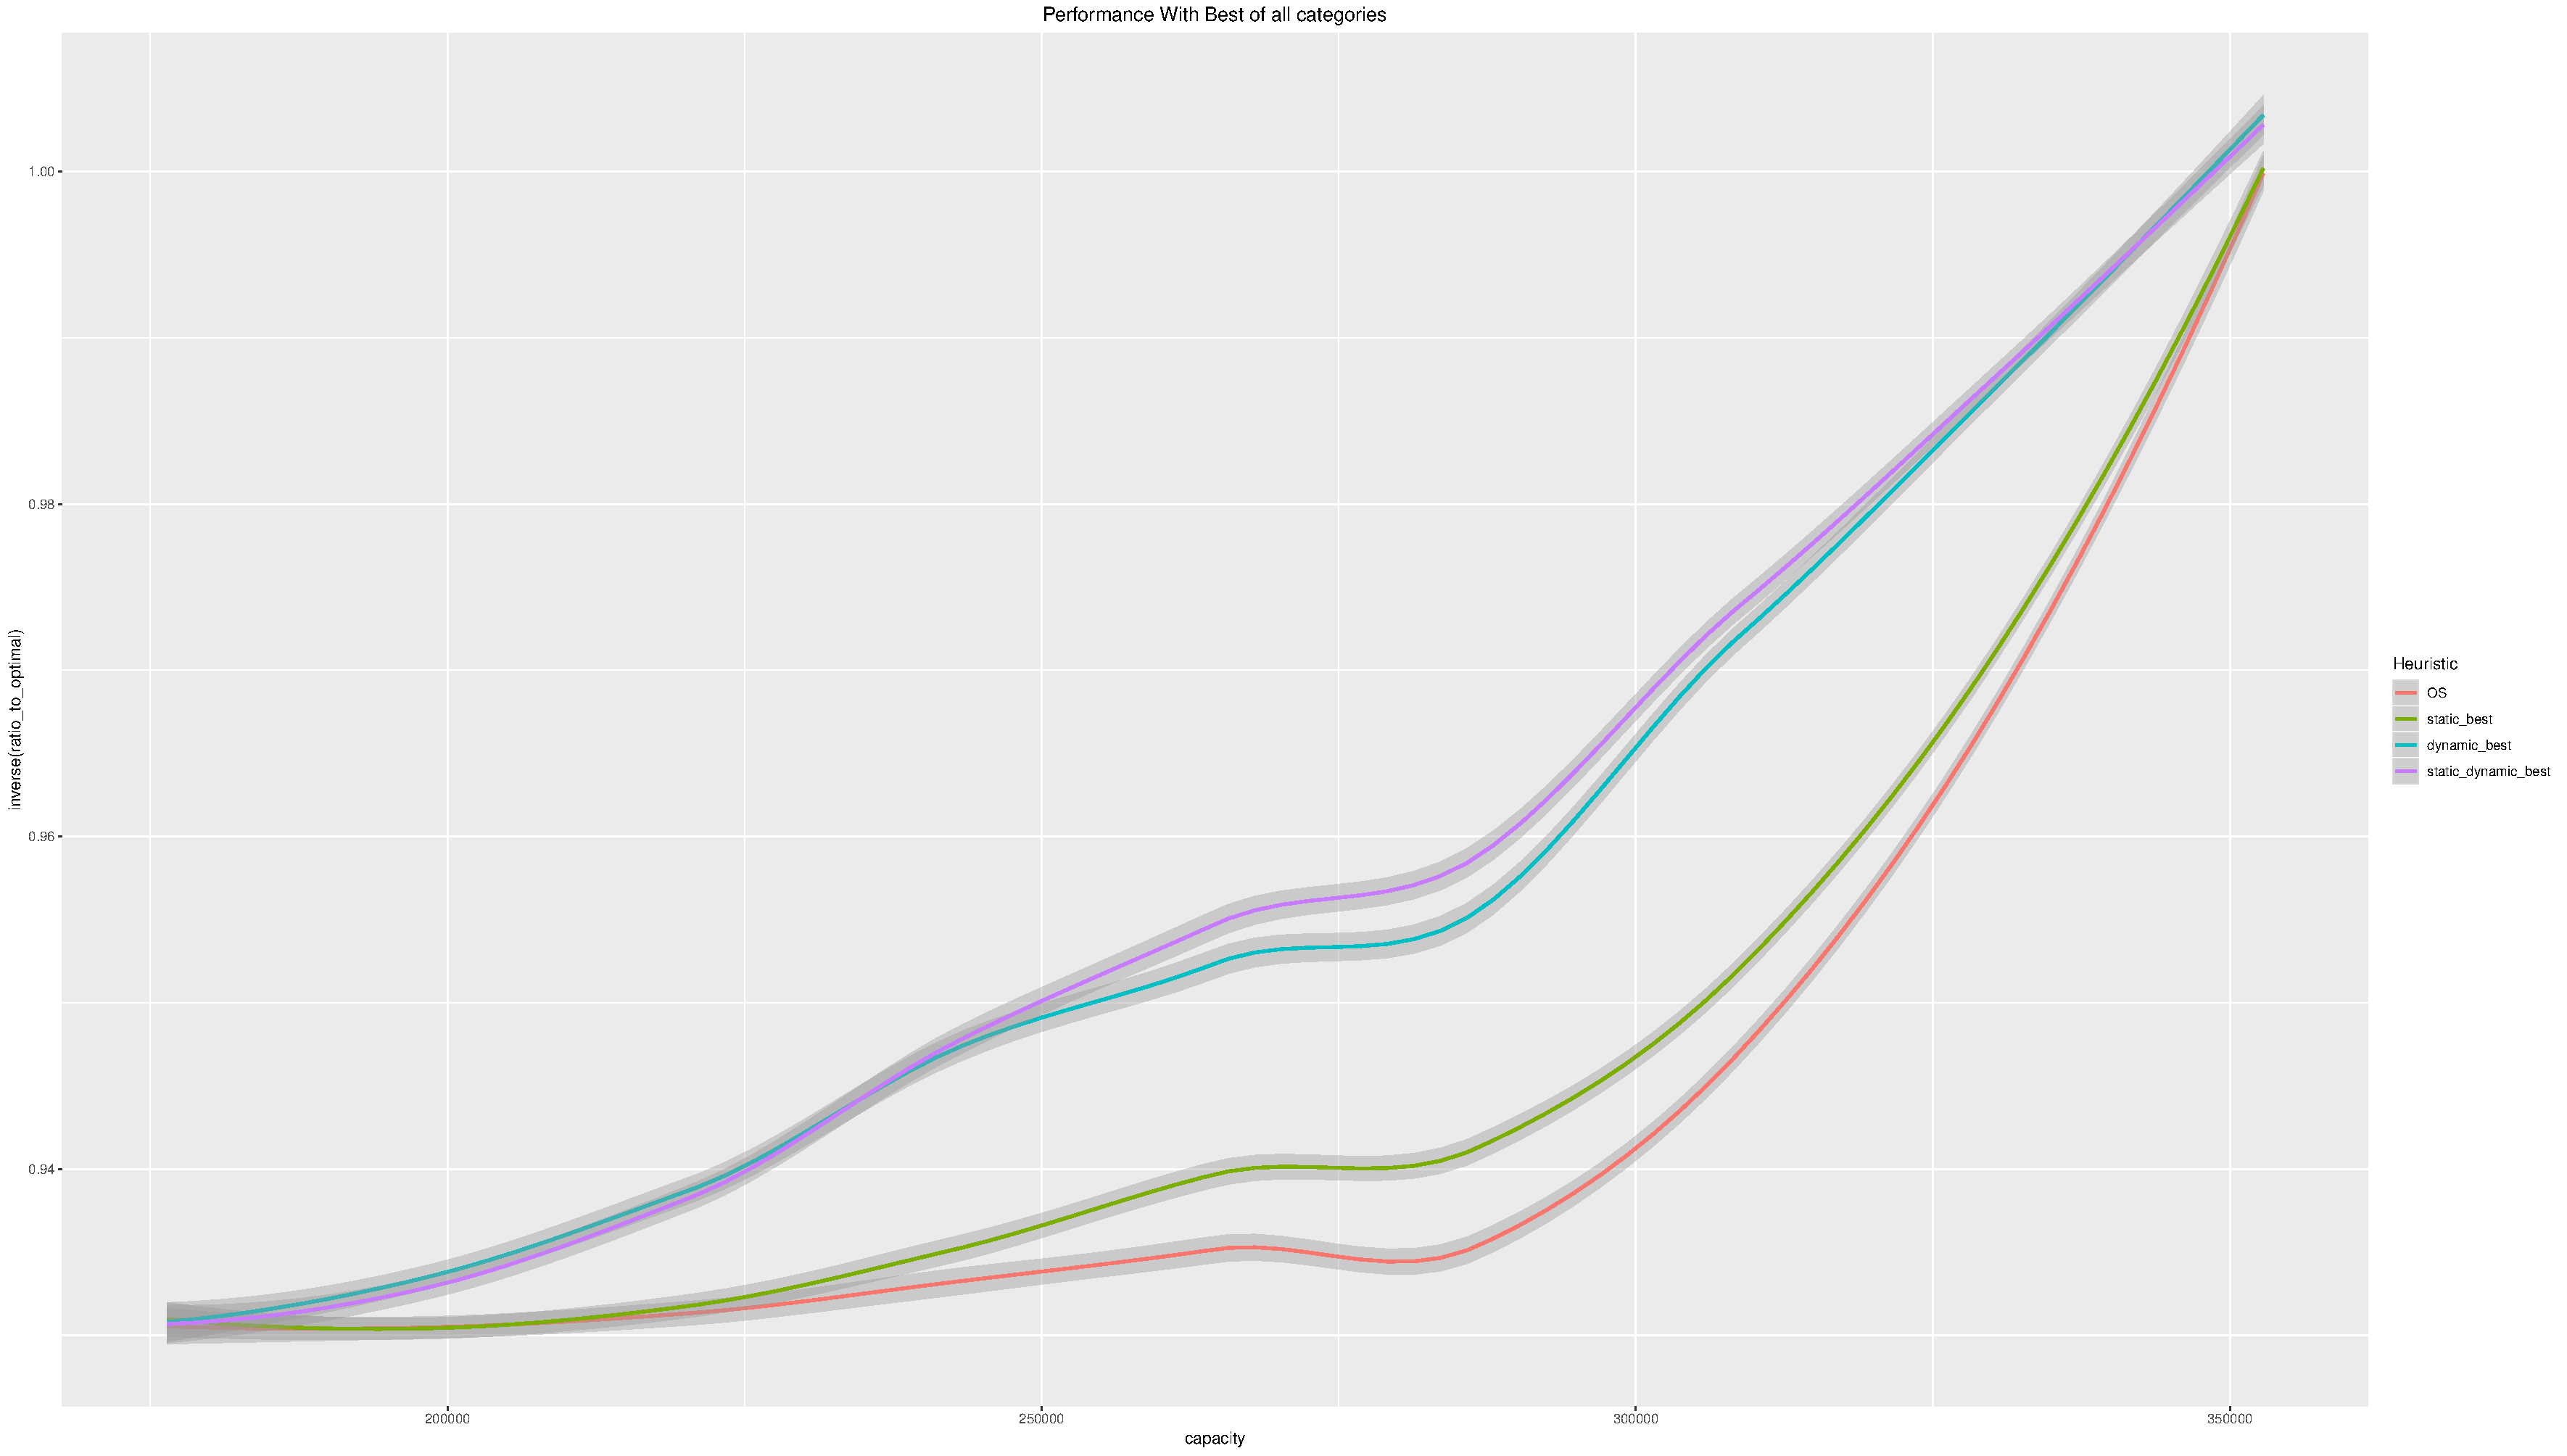
\includegraphics[scale=0.5]{./results/inverse_ratio_to_optimal_hf-best.pdf}
			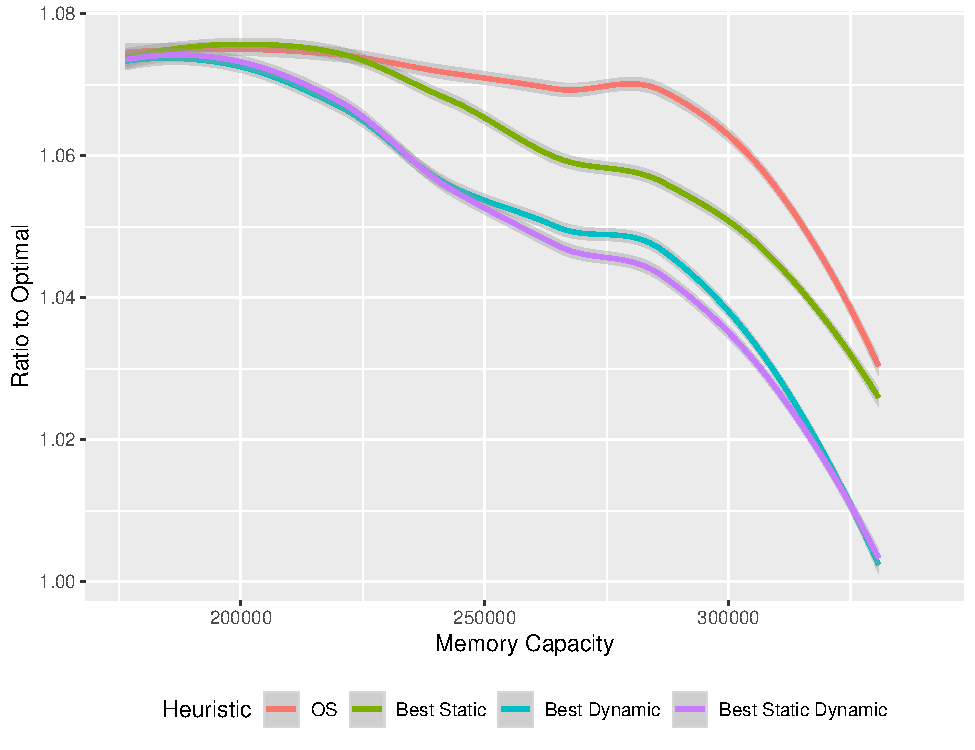
\includegraphics[scale=0.5]{./results/ratio_to_optimal_hf-best.pdf}
			\caption{Best variants of all categories for HF.}
			\label{fig:ratio_to_optimal_best_hf}
		\end{figure}
		
		
		Figure~\ref{fig:ratio_to_optimal_best_hf} shows the performance comparison of the best variant in each category, in addition to the \textit{order of submission} ($OS$) strategy which orders tasks in the (arbitrary) sequence in which they are given. Static strategies are expected to perform better when there is not any memory capacity restriction, and indeed this plot shows that static strategies face capacity bottleneck and underperform with limited memory. Dynamic strategies achieve slightly better performance with limited memory capacity, but when memory capacity is larger, static order with dynamic corrections strategies outperform all others.
		
		%%		\todo[inline]{SKumar: If you look at Figure~\ref{fig:ratio_to_optimal_best_hf} carefully,  in the beginning dynamics variants outperform others. This behavior is easily noticeable in Figure~\ref{fig:ratio_to_optimal_hf}. }
		%%		\todo[inline]{LED: Ok, I rephrased here a bit to mention this.}
		
		\subsection{CCSD Performance}
		\begin{figure*}[htb]
			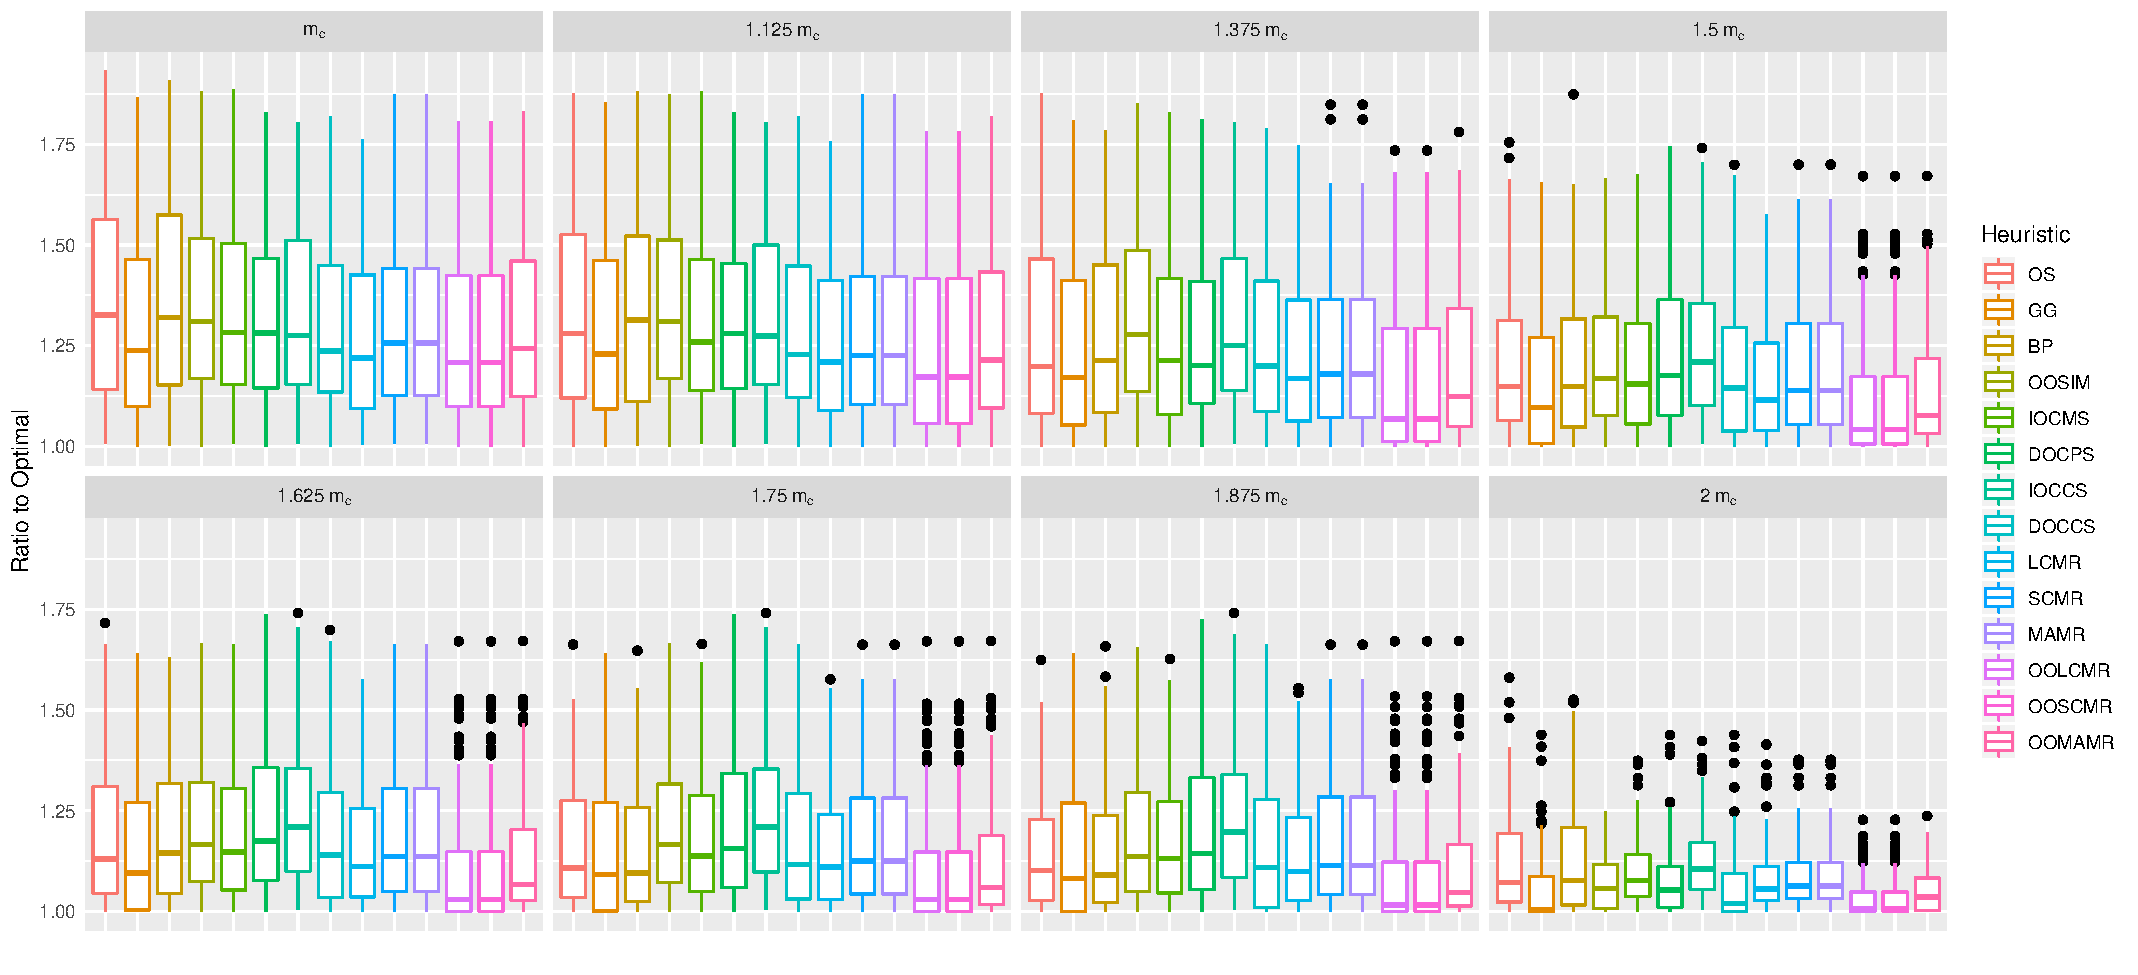
\includegraphics[scale=0.5]{./results/ratio_to_optimal_selected_ccsd.pdf}
			\caption{Comparison of different heuristics for CCSD with $m_c=1.8GB$.}
			\label{fig:ratio_to_optimal_ccsd}
		\end{figure*}	
		
		The CCSD application operates on tasks of different sizes, hence different heuristics exhibit distinct behaviors even at minimum memory capacity $m_c$. Heterogeneity favors dynamic strategies, as can be seen by the fact that both dynamic and static order with dynamic corrections based strategies perform better than static based strategies. Similar to HF, static order with dynamic corrections based strategies outperform others as memory capacity becomes moderate. 
		
		
		\begin{figure}[htb]
			%%			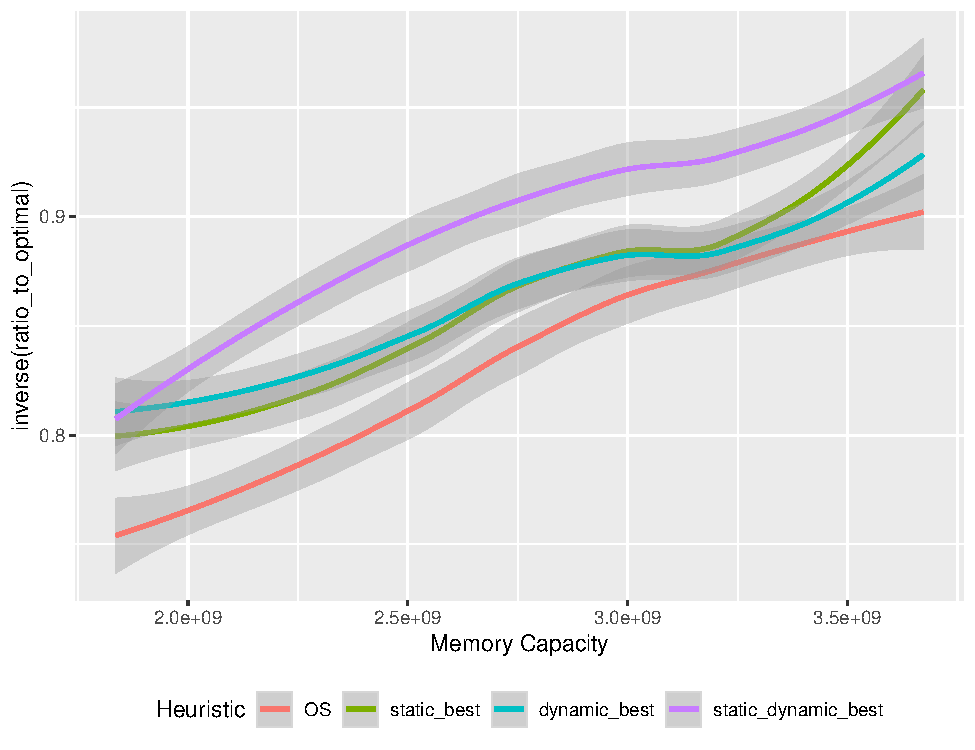
\includegraphics[scale=0.5]{./results/inverse_ratio_to_optimal_ccsd-best.pdf}
			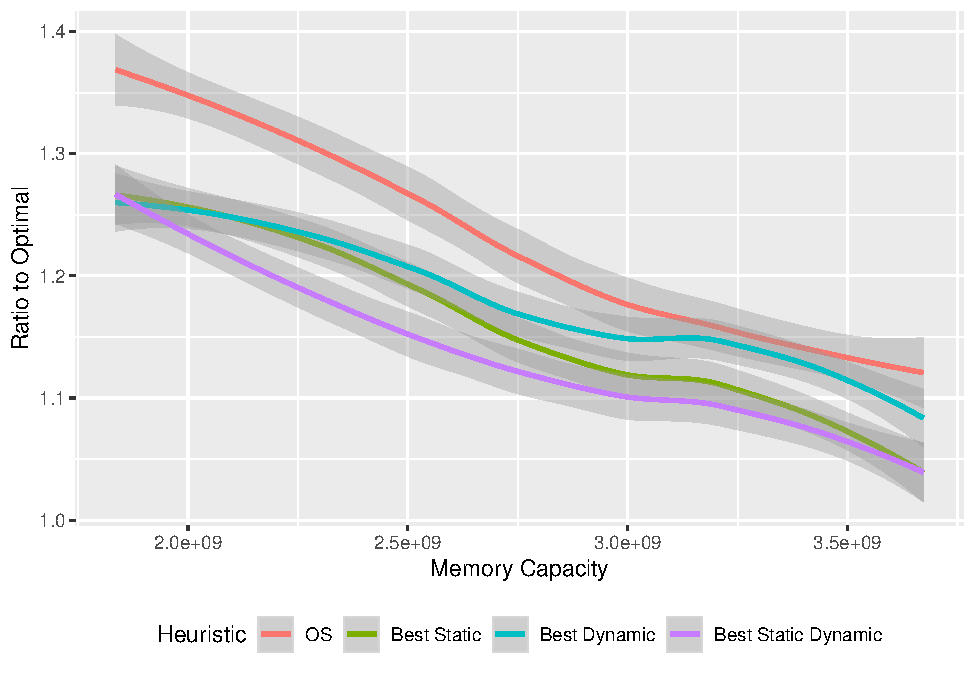
\includegraphics[scale=0.5]{./results/ratio_to_optimal_ccsd-best.pdf}
			\caption{Best variants of all categories for CCSD.}
			\label{fig:ratio_to_optimal_best_ccsd}
		\end{figure}
		
		Figure~\ref{fig:ratio_to_optimal_best_ccsd} shows that best variants of dynamic and static order with dynamic corrections strategies achieve similar performance at minimum memory capacity $m_c$. But as memory capacity increases, heterogeneity allows static order with dynamic corrections based strategies to take advantage of static knowledge to get maximum overlap and dynamic correction to select another task in case of memory capacity limitation. Static strategies also start performing better at the end, which indicates that this application has potential for significant communication-computation overlap and pure dynamic strategies are unable to take this information into account while making scheduling decisions.
		
		\subsection{Scheduling in Batches}
		In most applications, the runtime scheduler may only observe a limited batch of independent tasks. Therefore we organize tasks of each trace file in batches of 100 (the last batch may have less than 100 tasks). We apply each heuristic on each group in succession. Figure~\ref{fig:best_variants_batch} shows the performance of the best variant of each category for both applications. The plots exhibit behavior similar to Figures~\ref{fig:ratio_to_optimal_best_hf} and~\ref{fig:ratio_to_optimal_best_ccsd}: static order with dynamic corrections variants attain maximum communication-computation overlap and outperform other heuristics.
		
		\begin{figure*}[htb]
			%%			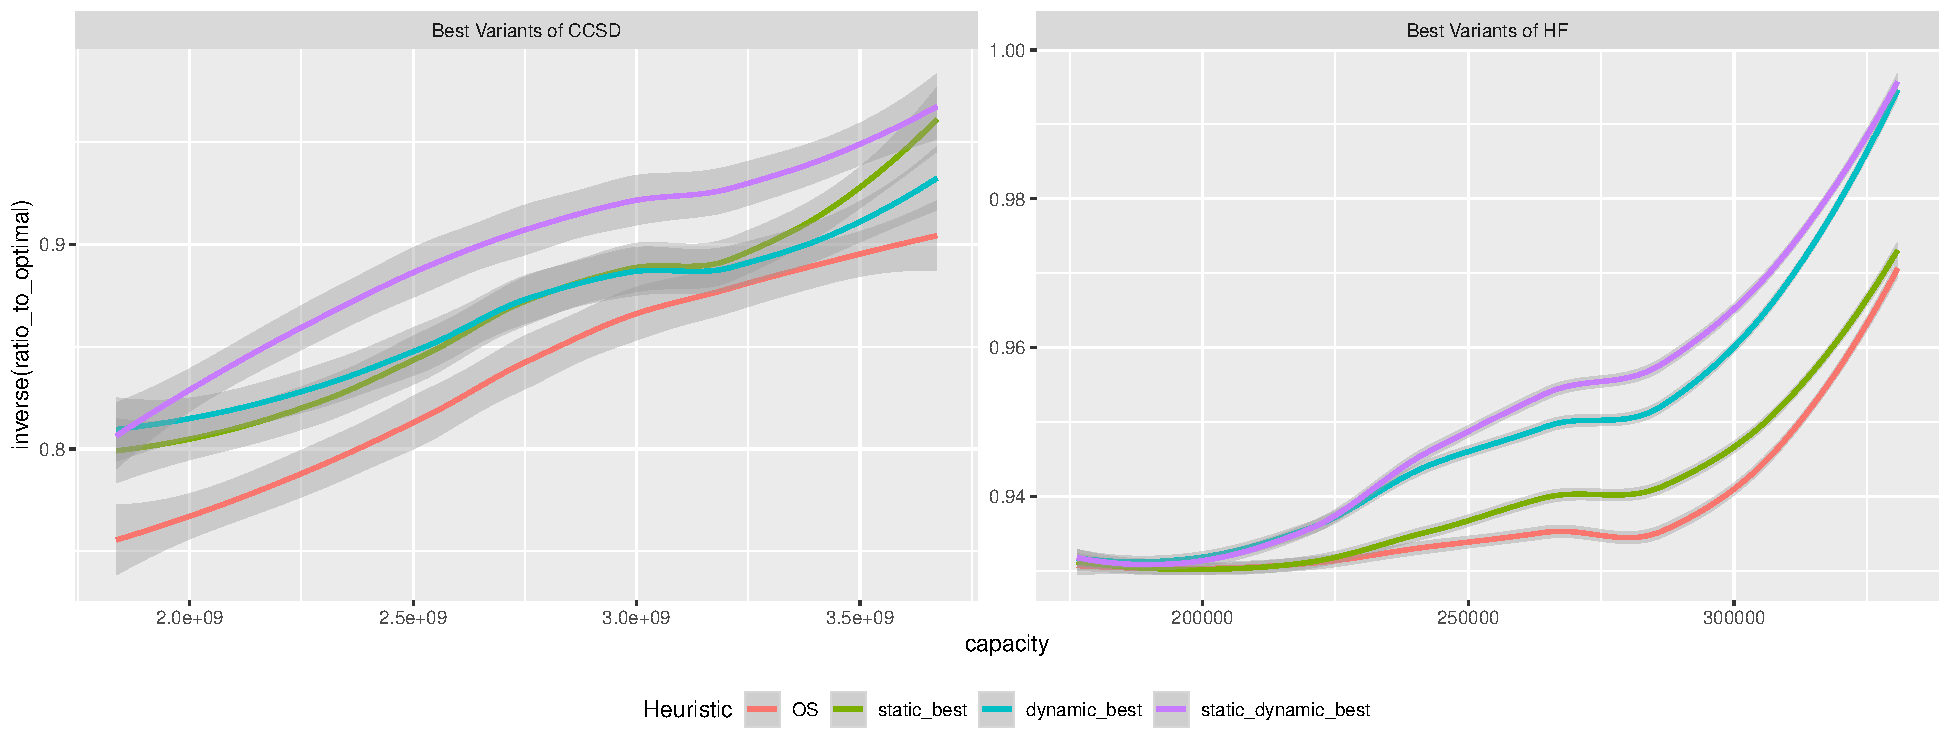
\includegraphics[scale=0.5]{./results/inverse_ratio_to_optimal_batch-best.pdf}
			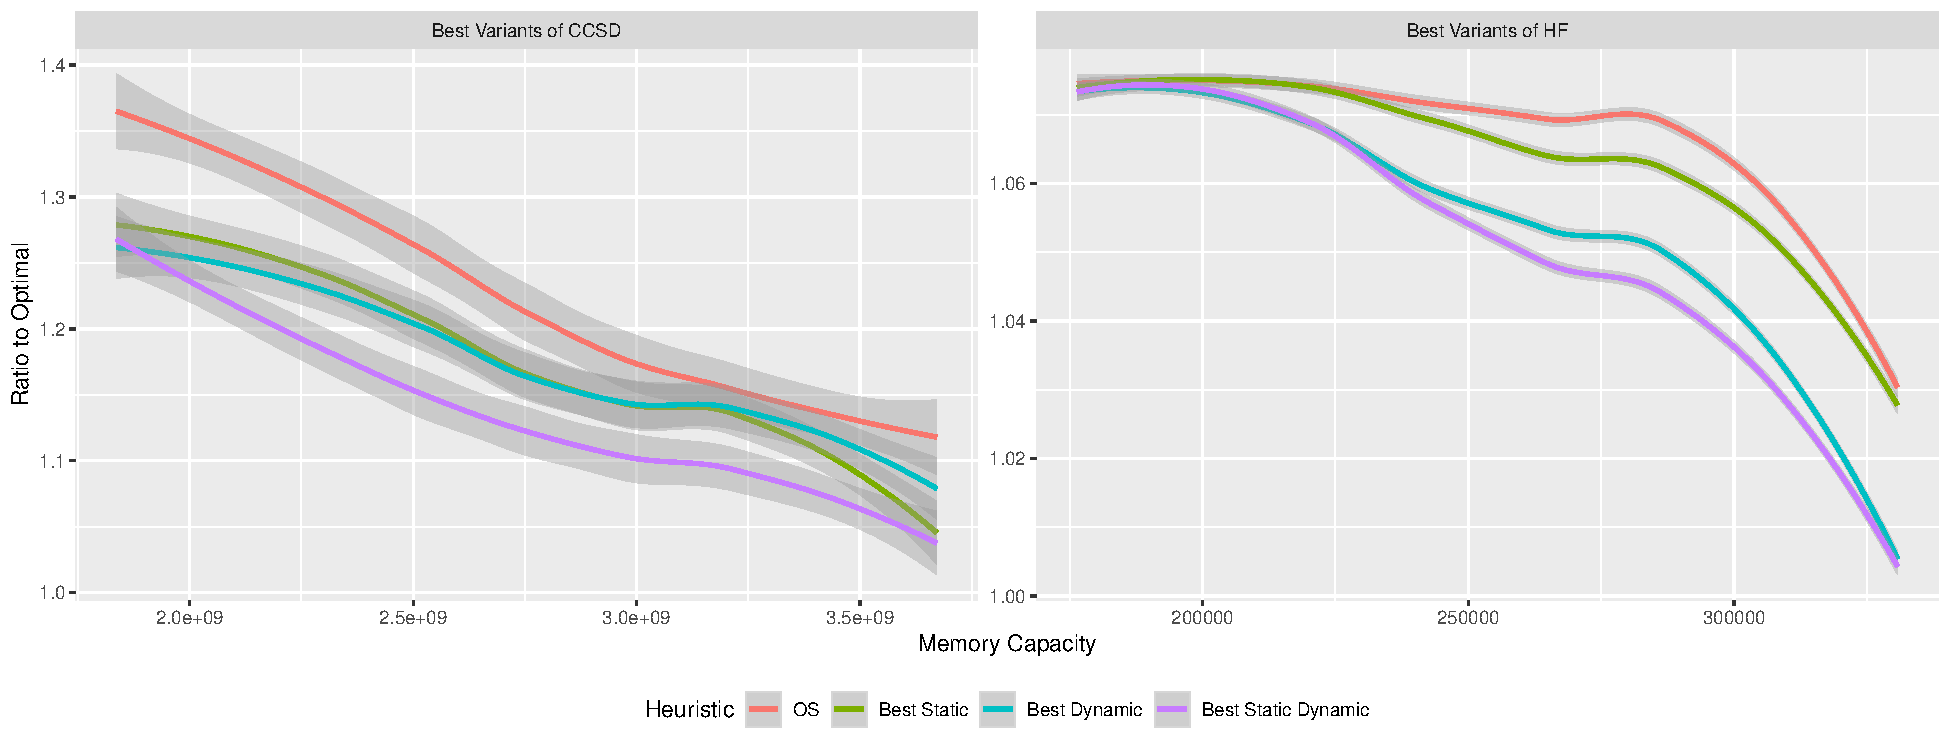
\includegraphics[scale=0.5]{./results/ratio_to_optimal_batch-best.pdf}
			\caption{Best variants of all categories where heuristics are applied in the batches of 100 tasks.}
			\label{fig:best_variants_batch}
		\end{figure*}
		
		
		
		%%\begin{figure}[htb]
		%%	\centering
		%%	\begin{subfigure}{.5\textwidth}
		%%		\centering
		%%		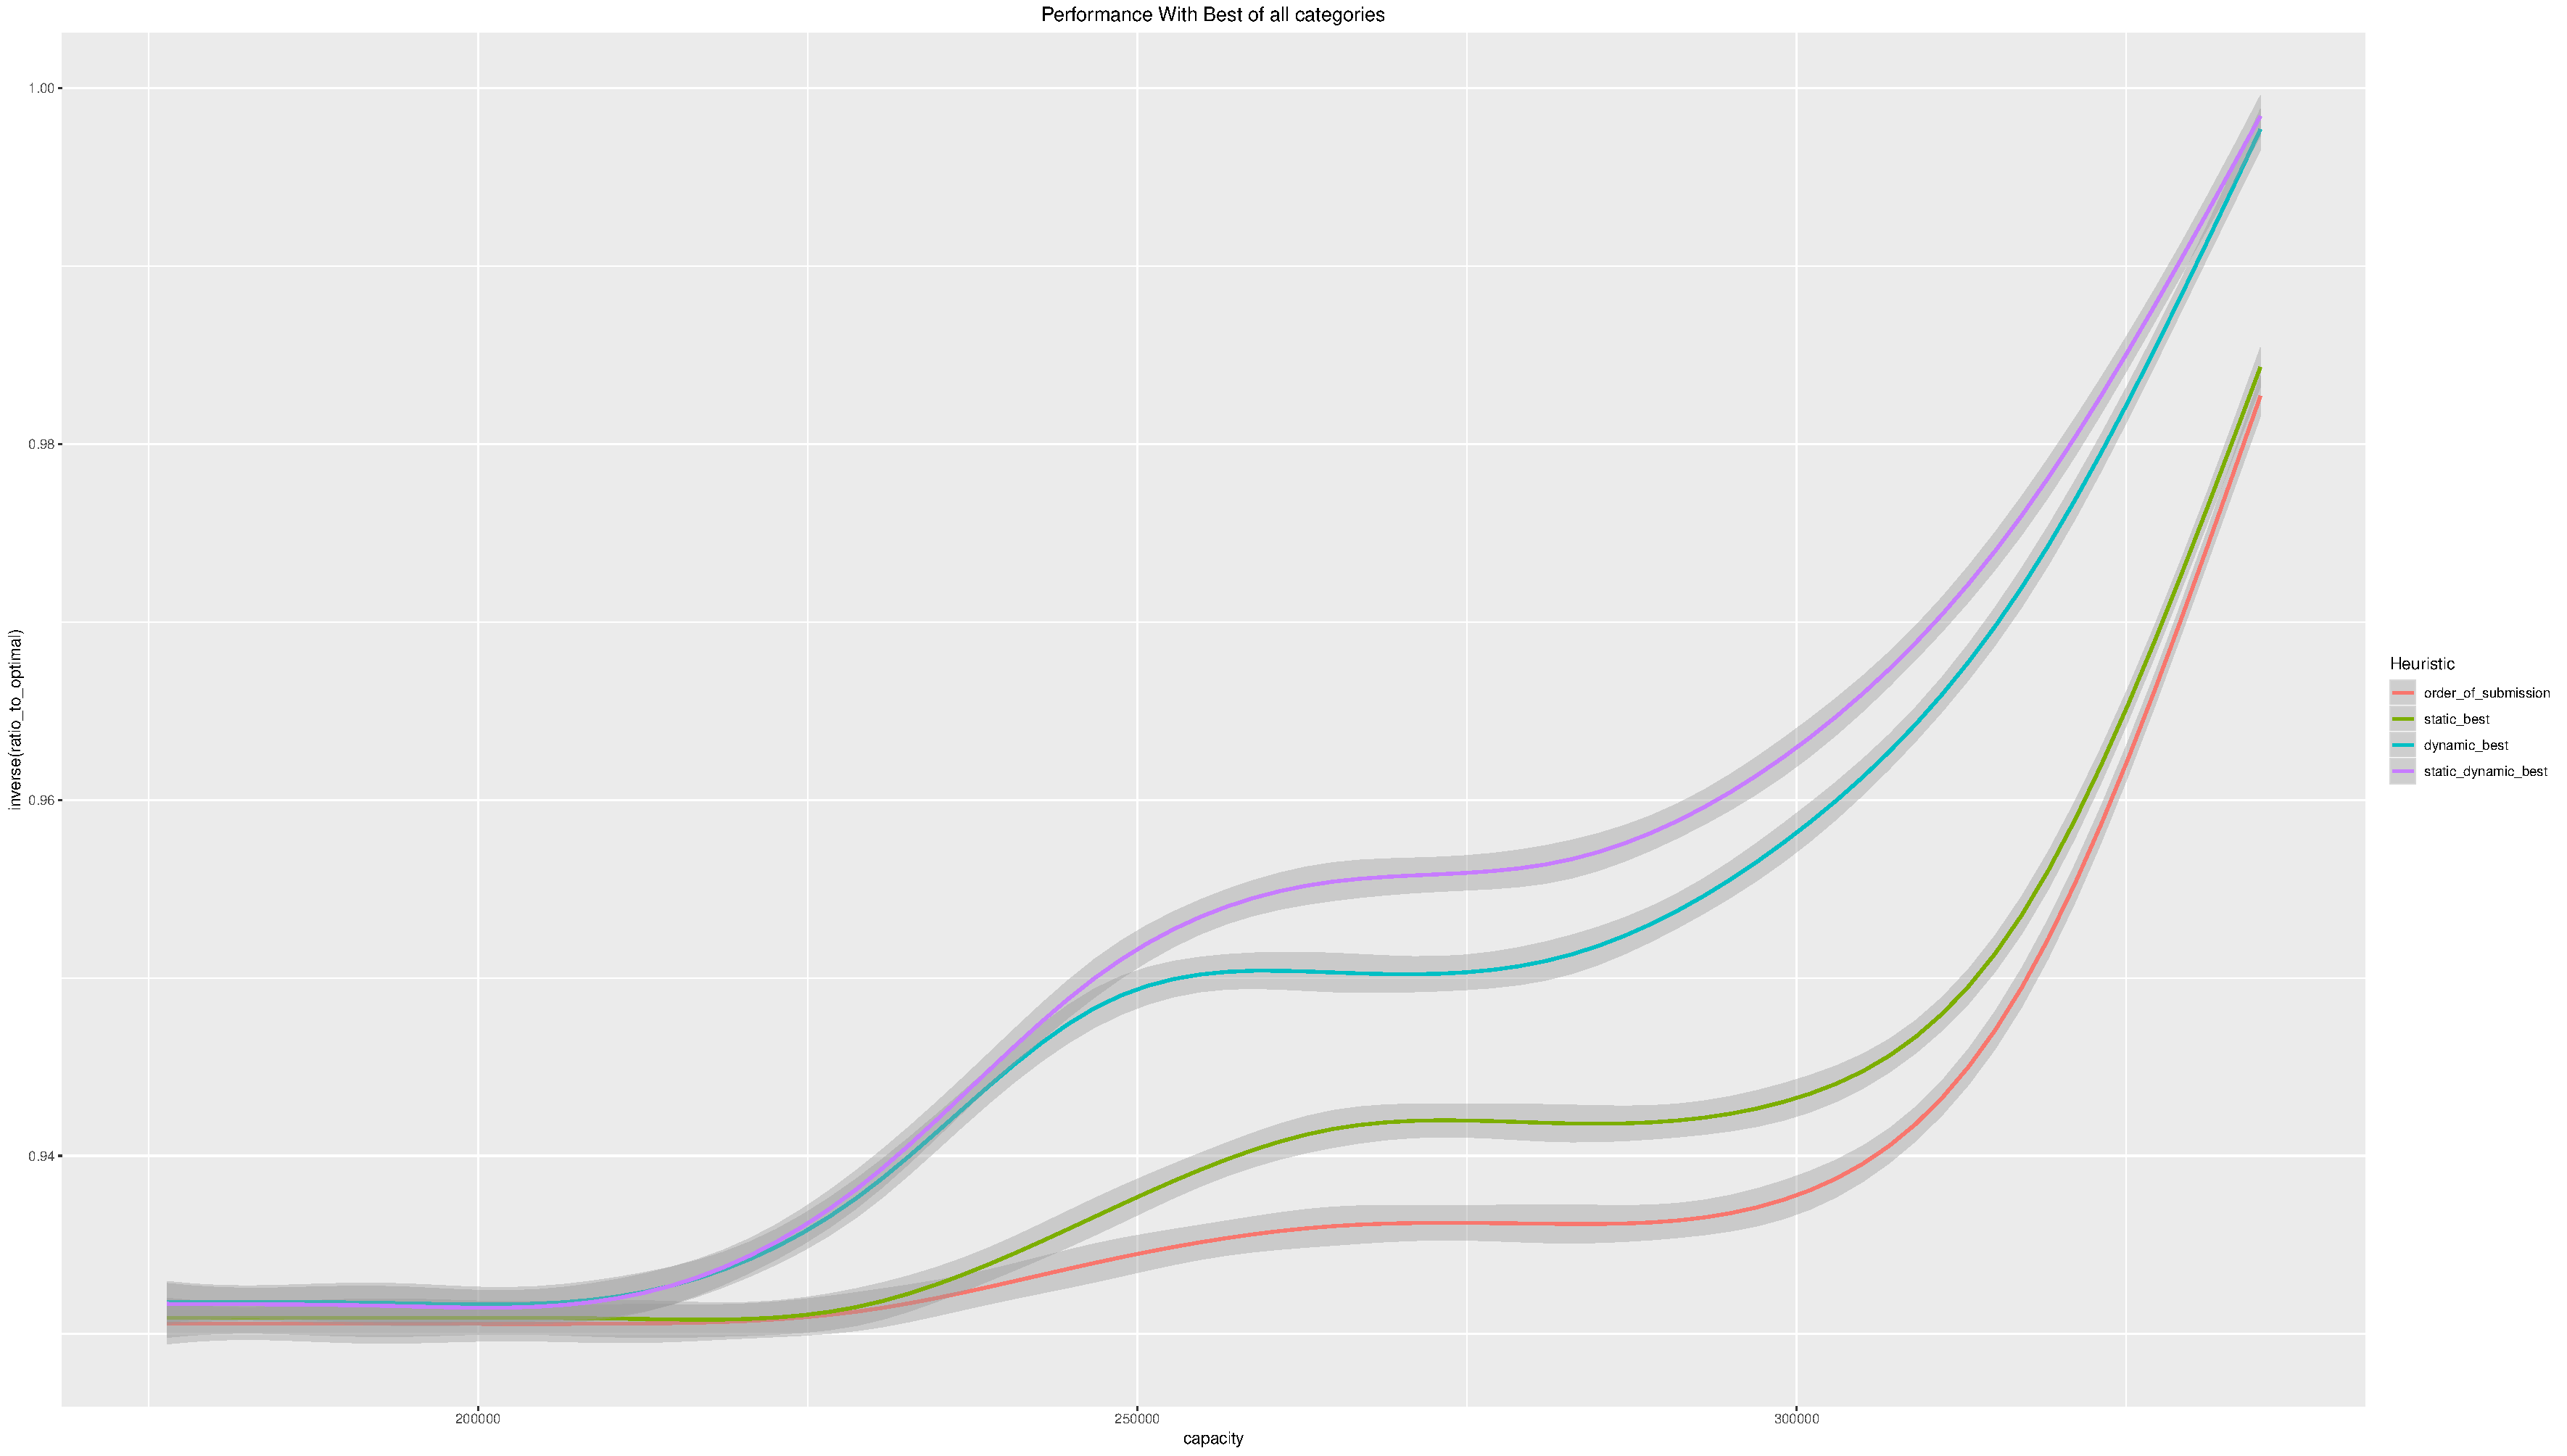
\includegraphics[width=.95\linewidth]{../ExperimentalResults/batch-100/inverse_ratio_to_optimal_hf_batch-best.pdf}
		%%		\caption{Best variants of HF.}
		%%		\label{fig:hf_best_variants_batch}
		%%	\end{subfigure}%
		%%	\begin{subfigure}{.5\textwidth}
		%%		\centering
		%%		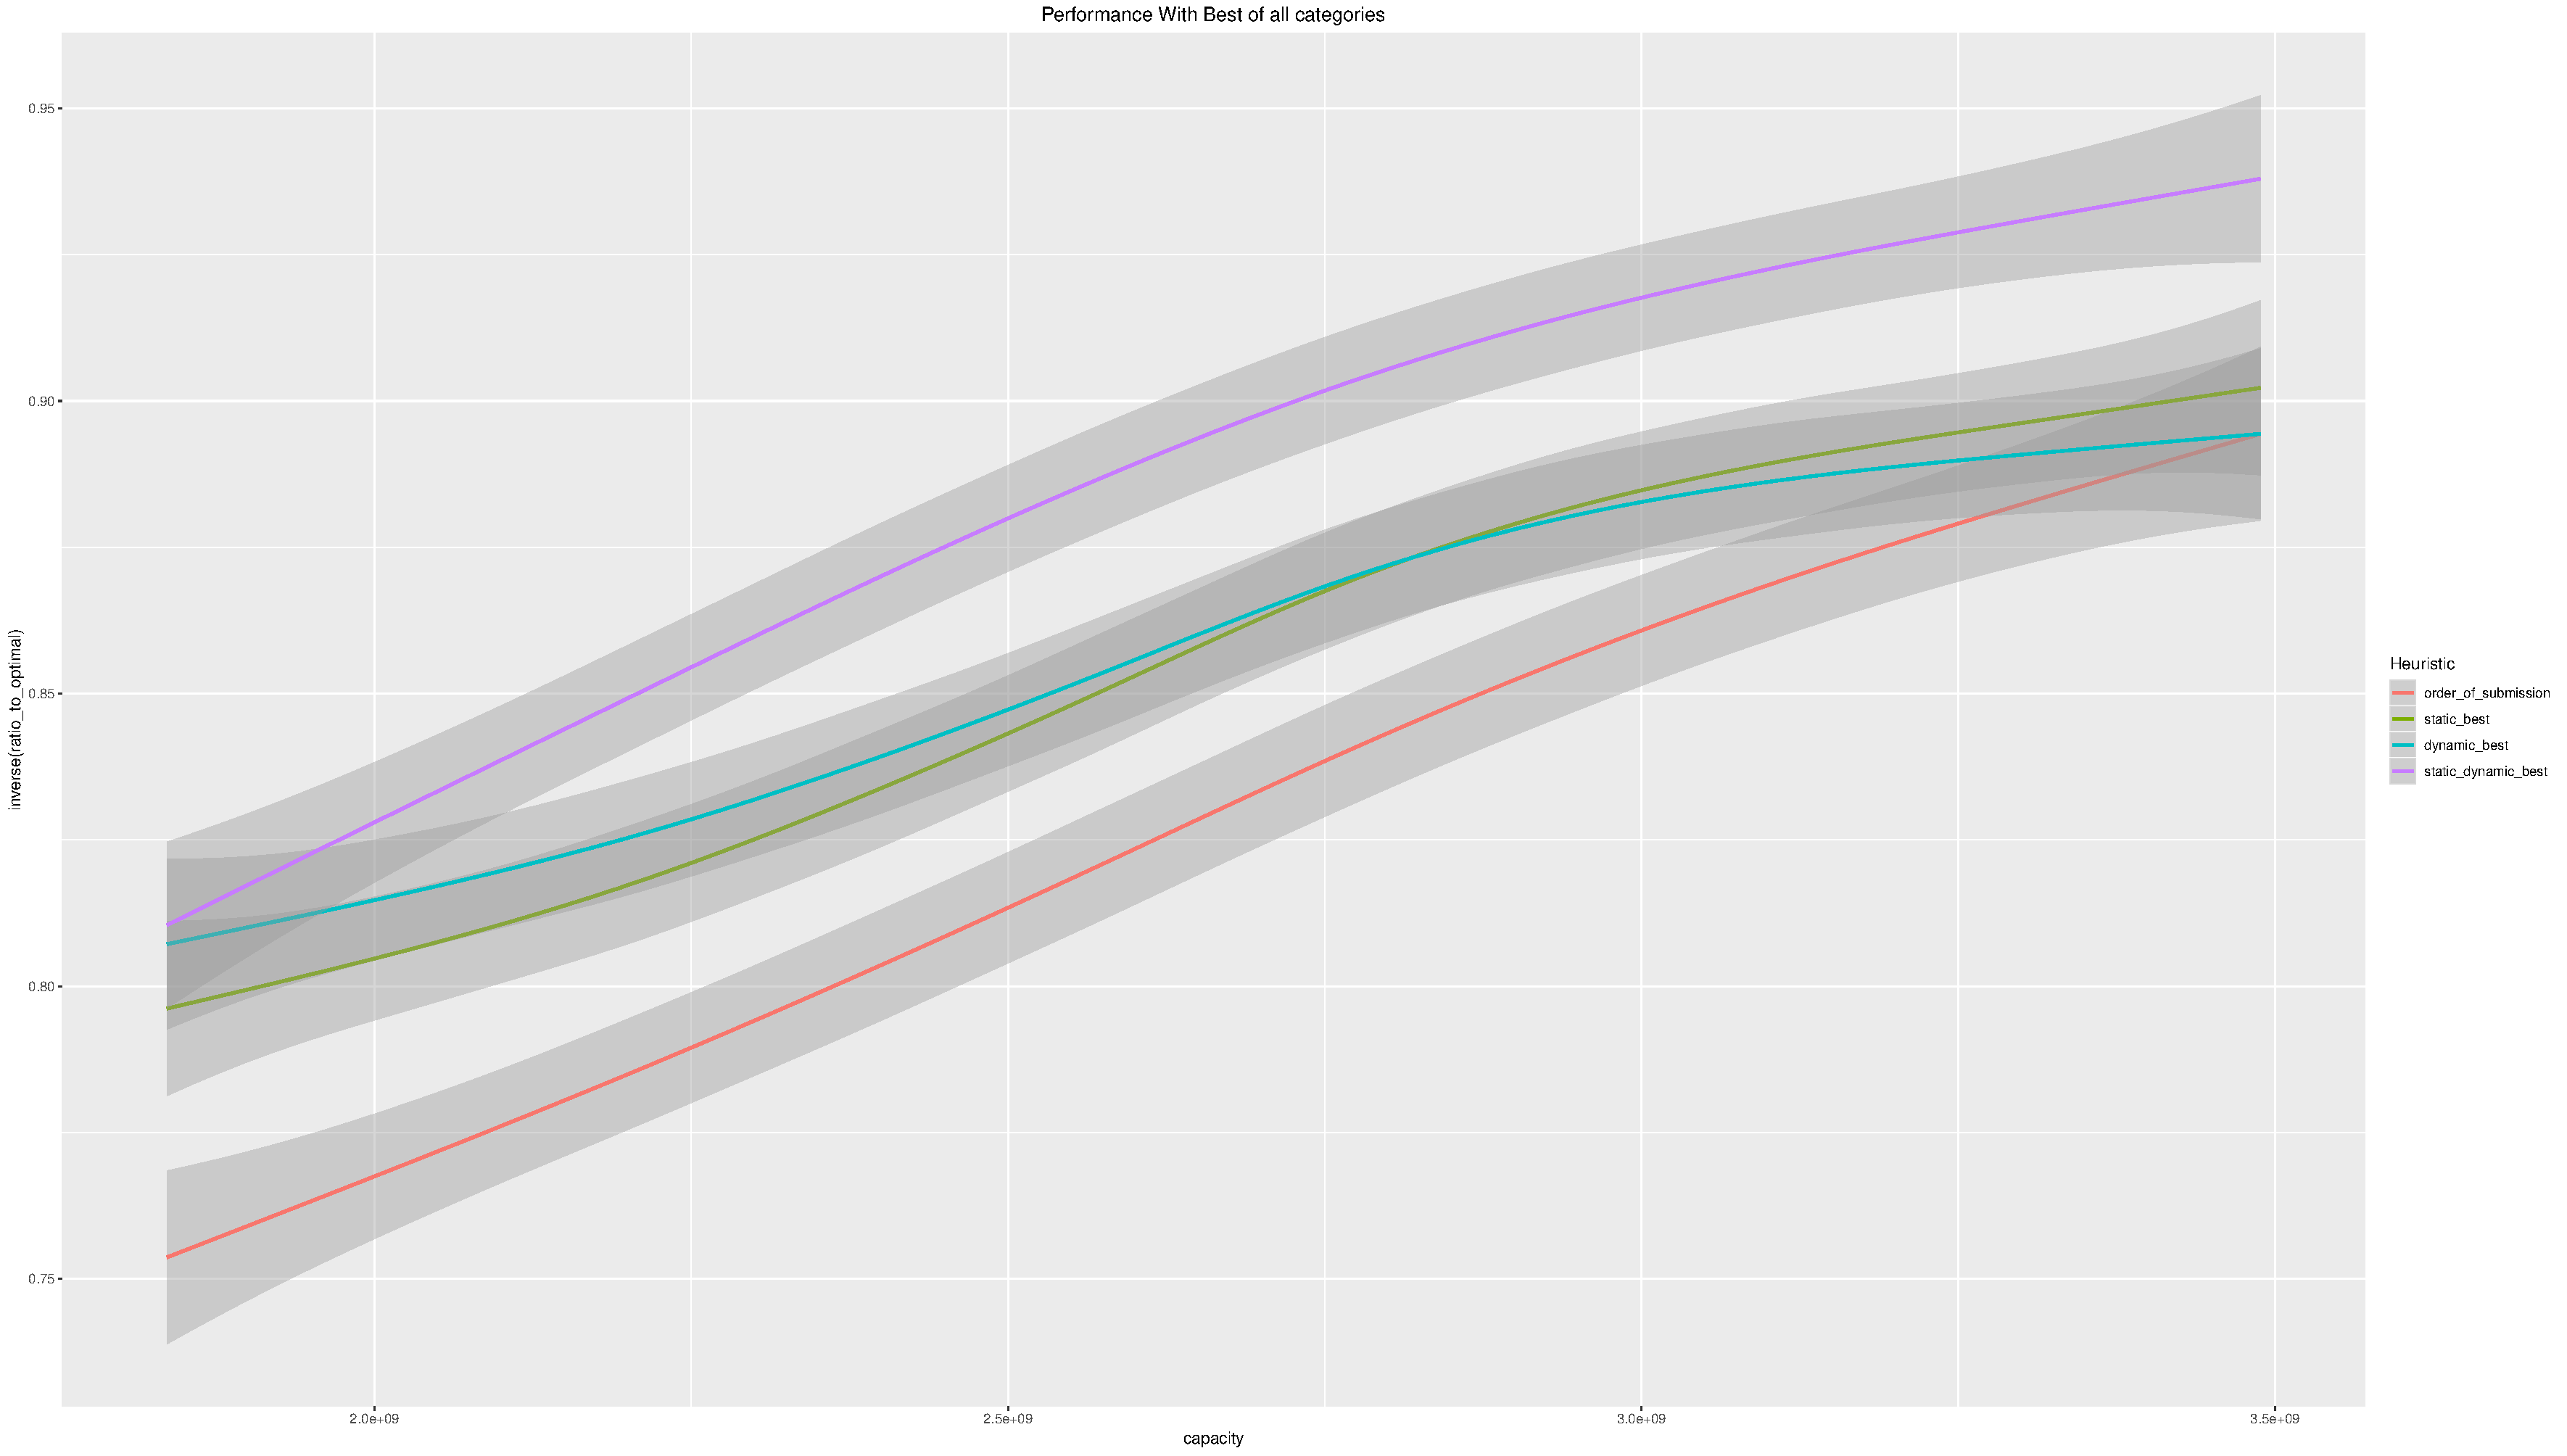
\includegraphics[width=.95\linewidth]{../ExperimentalResults/batch-100/inverse_ratio_to_optimal_ccsd_batch-best.pdf}
		%%		\caption{Best variants of CCSD.}
		%%		\label{fig:ccsd_best_variants_batch}
		%%	\end{subfigure}
		%%	\caption{Best variants of all categories where heuristics are applied in the batches of 100 tasks.}
		%%	\label{fig:best_variants_batch}
		%%\end{figure}
		
		%%	\subsection{Impact of heterogeneity on different heuristics}
		%%	\todo[inline]{SKumar: remove this subsection or replace with an experiment which shows the performance difference with all classes of heuristics for randomly generated inputs.}
		%%	\begin{figure*}[htb]
		%%		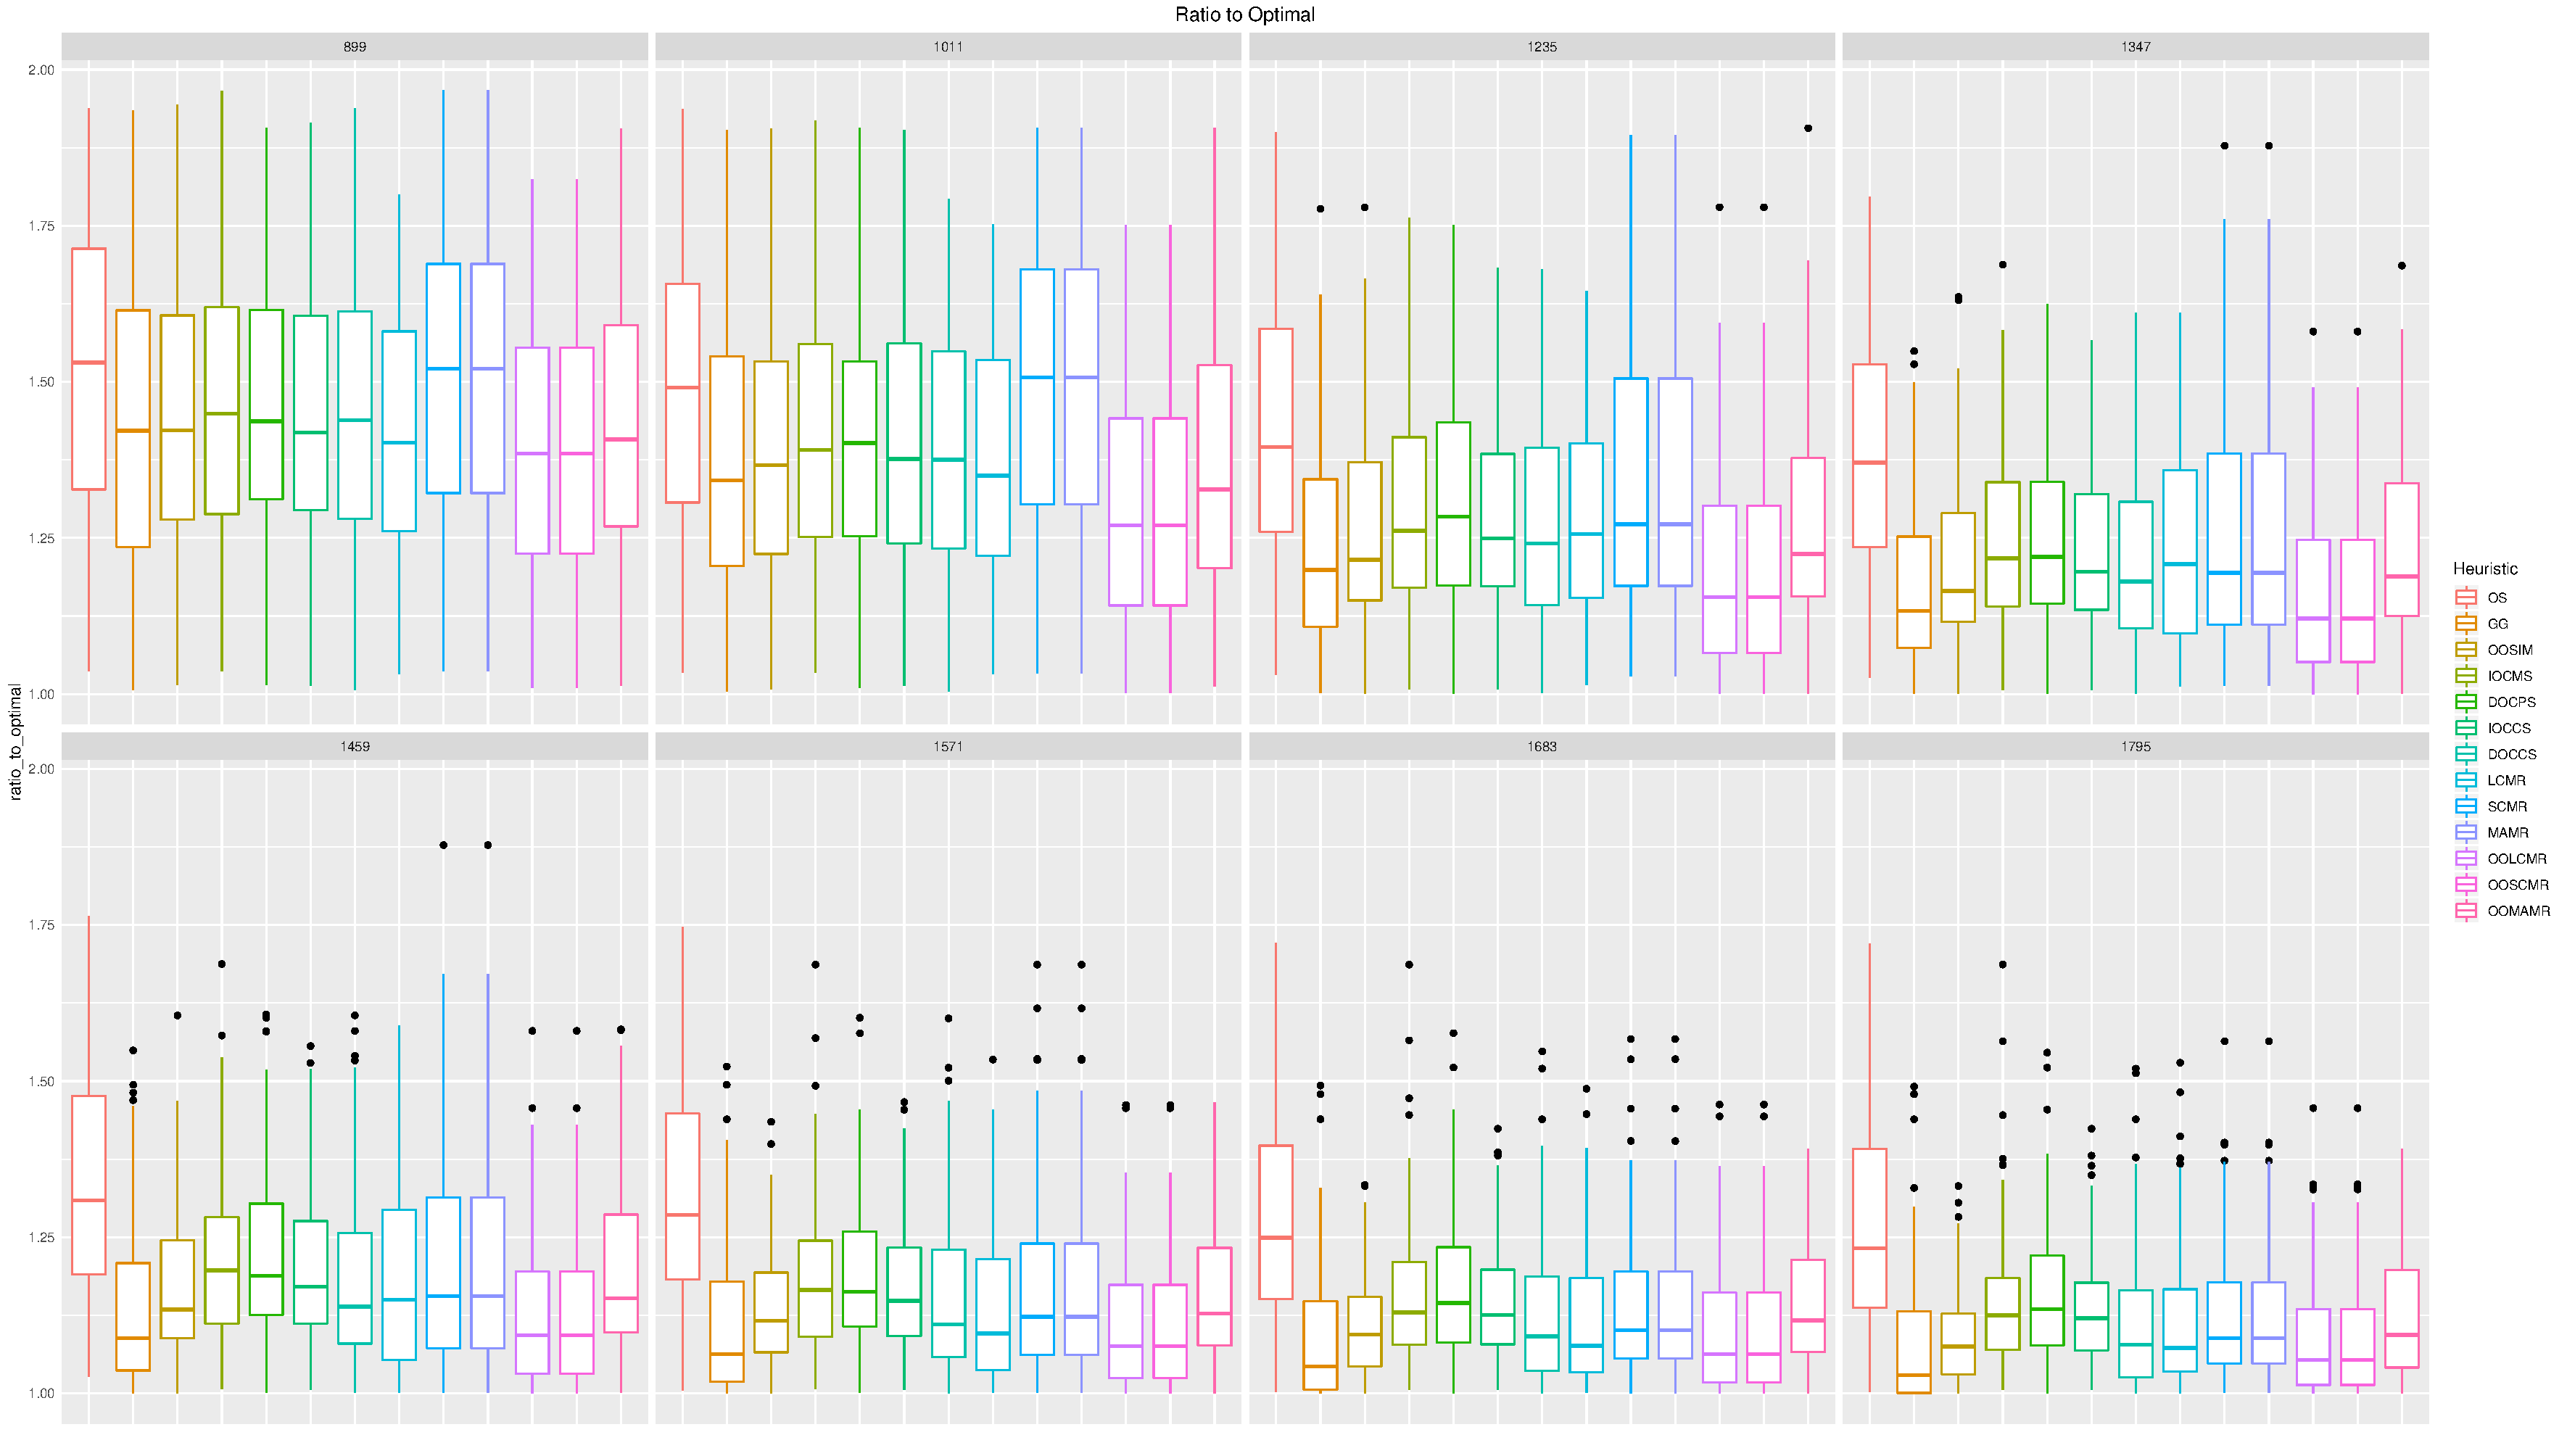
\includegraphics[scale=0.25]{./results/ratio_to_optimal_random_selected_ccsd.pdf}
		%%		\caption{Comparison of different heuristics for CCSD with highly heterogeneous tasks.}
		%%		\label{fig:ratio_to_optimal_ccsd_random}
		%%	\end{figure*}	
		%%	
		%%	
		%%	To know the affect of heterogeneity, we set the memory requirement of each task in CCSD trace randomly between 100 to 900 and observe the behavior of different heuristics in Figure~\ref{fig:ratio_to_optimal_ccsd_random}. This plot also exhibits that static order with dynamic correction variants make good use of static information to maximize communication-computation overlap and dynamic mechanism to minimize the penalty caused by memory capacity limitation. Pure static strategies suffer from memory capacity imitation and pure dynamic strategies are unable to maximize communication-computation overlap.
		
		
		\section{Conclusion and Perspectives}
		\label{sec:conclusion}
		
		%%We also plan to extend our model by taking bandwidth sharing and different possible routes for the same source-destination pair into account.
		
		In this paper, we consider the problem of deciding the order of data transfers between two memory nodes such that overlap of communications and computations is maximized. With Exascale computing, applications face bottlenecks due to communications. Hence, it is extremely important to achieve the maximum  communication-computation overlap in order to exploit the full potential of the system. We show that determining the order of data transfers is a NP complete problem. We propose several data transfer heuristics and evaluate them on two molecular chemistry kernels, HF and CCSD. Our results show that some of our heuristics achieve significant overlap and perform very close to the lower bound. We plan to evaluate our strategies on different applications coming from multiple domains. We also plan to study the behavior of our strategies in the context of overlapping CPU-GPU communications with computations. A runtime system aiming at exposing different heuristics to maximize the communication-computation overlap at the developer level and automatically selecting the best one is currently underway.
		
		
		\begin{acks}
			
			We are grateful to Ajay Panyala for his help in installation of  NWChem on Cascade machine and providing internal details about the package and its inputs. This work was supported in part by the U.S. Department of Energy (DOE), Office of Science, Office of Advanced Scientific Computing Research, under award 63823. Pacific Northwest National Laboratory is operated by Battelle for DOE under Contract DE-AC05-76RL01830.
		\end{acks}
		
		%
		% The next two lines define the bibliography style to be used, and the bibliography file.
		\bibliographystyle{ACM-Reference-Format}
		\bibliography{communications}
		
	\end{document}
